%%
%% patent_analysis_tool.tex — Programmatic Patent Analysis Environment
%% CS 294-184 Final Project Part 2
%% Based on sample-sigconf-authordraft.tex from the acmart package.
%%
\documentclass[sigconf]{acmart}
\usepackage{graphicx}
\usepackage{microtype}
\usepackage{listings}
\usepackage{needspace}
\usepackage{xcolor}
\emergencystretch=1em

%%
%% \BibTeX command to typeset BibTeX logo in the docs
\AtBeginDocument{%
  \providecommand\BibTeX{{%
    Bib\TeX}}}

%% Rights management information.
\setcopyright{acmlicensed}
\copyrightyear{2026}
\acmYear{2026}
\acmDOI{XXXXXXX.XXXXXXX}

%% These commands are for a PROCEEDINGS abstract or paper.
\acmConference[Conference acronym 'XX]{Make sure to enter the correct
  conference title from your rights confirmation email}{June 03--05,
  2018}{Woodstock, NY}
\acmISBN{978-1-4503-XXXX-X/2018/06}

%% Listings style for DSL code examples
\lstdefinelanguage{PatentDSL}{
  morekeywords={AND, OR, NOT, section, contains, cpc, meta, paragraph, claim, figure, heading, sectionTitle, synonym_of, termset},
  sensitive=false,
  morestring=[b]",
}
\lstset{
  language=PatentDSL,
  basicstyle=\ttfamily\footnotesize,
  keywordstyle=\bfseries,
  stringstyle=\color{gray},
  frame=single,
  breaklines=true,
  breakatwhitespace=false,
  columns=fullflexible,
  keepspaces=true,
  captionpos=b,
}

\newcommand{\DocSectionPassage}{\texttt{Document} $\to$ \texttt{Section} $\to$ \texttt{Passage}}

%%
%% Start of document
%%
\begin{document}

\title{A Programmatic Patent Analysis Environment for Structured Prior-Art Search and Claim-Chart Drafting}

\author{Shanaya Malik}
\email{shanaya_malik@berkeley.edu}
\affiliation{%
  \institution{University of California, Berkeley}
  \city{Berkeley}
  \state{California}
  \country{USA}}

\author{Kelvin Zhao}
\email{kelvinyz@berkeley.edu}
\affiliation{%
  \institution{University of California, Berkeley}
  \city{Berkeley}
  \state{California}
  \country{USA}}

\renewcommand{\shortauthors}{Malik \& Zhao}

%% ====================================================================
%%  ABSTRACT
%% ====================================================================
\begin{abstract}
Patent examination requires experts to move repeatedly between corpus scoping,
targeted search, close reading, and claim-to-evidence mapping, but current
tools largely return ranked documents and leave section selection, citation
recovery, and claim-chart drafting to manual work. To understand what a better
abstraction should support, we conducted a contextual inquiry study with ten
practicing patent examiners and found recurring needs for section-aware
retrieval, pinpoint citation, iterative query refinement, and tighter
integration between search and synthesis. We present a programmatic patent
analysis environment that addresses these needs by representing each patent as
a structured \DocSectionPassage{} hierarchy,
exposing a composable passage-level DSL over structural, textual, and metadata
predicates, and preserving provenance as results move into a connected
evidence-capture workspace. Our prototype combines a FastAPI backend, a query
execution model over parsed patent passages, and a React frontend for corpus
scoping, live refinement, and lightweight claim-chart drafting. The paper
contributes the design rationale, implementation, and technical challenges of
treating prior-art search as an inspectable, programmable workflow rather than
ad hoc document inspection.
\end{abstract}

\begin{CCSXML}
<ccs2012>
 <concept>
  <concept_id>10003120.10003121.10003122.10010853</concept_id>
  <concept_desc>Human-centered computing~Empirical studies in HCI</concept_desc>
  <concept_significance>500</concept_significance>
 </concept>
 <concept>
  <concept_id>10003120.10003121.10003124.10010870</concept_id>
  <concept_desc>Human-centered computing~HCI design and evaluation methods</concept_desc>
  <concept_significance>300</concept_significance>
 </concept>
 <concept>
  <concept_id>10011007.10011006.10011008.10011009.10011012</concept_id>
  <concept_desc>Software and its engineering~Functional languages</concept_desc>
  <concept_significance>300</concept_significance>
 </concept>
</ccs2012>
\end{CCSXML}

\ccsdesc[500]{Human-centered computing~Empirical studies in HCI}
\ccsdesc[300]{Human-centered computing~HCI design and evaluation methods}
\ccsdesc[300]{Software and its engineering~Domain-specific languages}

\keywords{patent examination, prior art search, domain-specific language,
document analysis, contextual inquiry, sensemaking, information work, HCI}

\maketitle


%% ====================================================================
%%  SECTION 1 — MOTIVATION  (1–2 pages)
%% ====================================================================
\section{Motivation}

\smallskip\noindent\textbf{The stakes of patent examination.}
Patent examination is a high-stakes, knowledge-intensive activity in which
trained examiners must locate prior art---existing patents, publications, or
other disclosures---that \emph{anticipates} or \emph{obviates} each claim in a
pending patent application. Because issued patents carry legal force, the
quality of examination directly affects the validity of the intellectual
property record and the downstream costs of litigation and re-examination.
Yet the core task of finding prior art remains largely manual: an examiner
reads the claims, identifies the key technical concepts, formulates search
queries, retrieves candidate documents, reads those documents to find relevant
passages, and then records exactly \emph{where} in each document the evidence
appears so it can be cited in an office action. For complex technical art
units---software, biomedical devices, quantum computing---this cycle can span
dozens of documents and hundreds of individual claim elements per application.

\smallskip\noindent\textbf{Why existing tools are insufficient.}
Current search infrastructure, including the USPTO's internal EAST and WEST
systems as well as commercial tools such as PatSnap and Derwent Innovation,
treats this workflow at the document level. A query returns a ranked list of
patent documents; the examiner then opens each document and manually locates
the relevant section. Tools surface keyword hit \emph{counts}, but do not
distinguish whether a hit appears in the abstract, the background, the
detailed specification, or the claims---sections that carry very different
evidentiary weight. Passage-level retrieval, section-aware filtering, and
metadata-constrained queries are not available as first-class capabilities in
any tool accessible to working examiners.

\smallskip\noindent\textbf{Evidence from practitioners.}
Through a contextual inquiry study with ten practicing patent examiners (reported
in full in Sections~3--4), we identified five recurring needs that current
tooling does not address: synonym generation, filing-date filtering,
claim-mapping handoff, section-aware passage inspection, and iterative query
refinement. These are not edge cases. They recur inside the ordinary path from
reading a claim to writing an office action. For example, P05 explicitly wanted
hits in the background and detailed description sections rather than the
abstract or claims, because the specification is where the technical teaching
that maps to claim elements is typically found. P03 showed that determining
which references were even legally admissible could require tedious manual date
inspection across candidate documents. P01 emphasized the effort required to
recover exact paragraph-level locations for later citation, and multiple
participants described the move from search into claim mapping as a separate,
mostly manual activity carried out in Word, paper notes, or personal templates.
Taken together, these observations make the need important not just because the
workflow is slow, but because critical legal-technical judgments are being made
through brittle manual transitions.

\smallskip\noindent\textbf{The root cause: documents as opaque blobs.}
A further structural problem unifies all five needs: patent documents are
treated as opaque text blobs. Queries operate over full-text indexes; results
are document-level rankings. The rich internal structure of a patent---its
sections, numbered paragraphs, claim hierarchy, and embedded
metadata---is invisible to the query layer. An examiner who wants to find all
passages in the detailed specification of a particular assignee's patents that
discuss a specific technical mechanism must open each document, scroll to the
relevant section, and scan manually. This is not a failure of individual tools
but a consequence of the retrieval model: when documents are the unit of
retrieval, there is no path to passage-level precision.

\smallskip\noindent\textbf{Why this gap persists.}
This problem has been hard to solve because patent search is usually framed as a
retrieval problem rather than a workflow problem. Existing systems compete on
coverage, ranking, and document access, which makes sense if the main question
is which references to open next. Our study suggests that this framing is too
narrow for examiner work. Examiners do not stop at document retrieval: they
must interpret where relevant teaching appears, verify admissibility, preserve
citation anchors, and organize evidence against claim elements. Those steps cut
across information retrieval, document structure, and downstream synthesis, so
they tend to fall between existing tool categories. The workflow is also hard to
study directly because much examiner practice happens inside specialized,
institutional settings and proprietary tool ecosystems, which means the
downstream coordination work is easier to miss than the search box itself.

\smallskip\noindent\textbf{Our approach and expected outcomes.}
We propose a different approach. Rather than building another document-level
search interface, we present a \emph{programmatic patent analysis environment}
that combines corpus scoping, structured passage-level querying, and evidence
capture for claim-chart drafting. The environment parses each patent into a
\DocSectionPassage{} hierarchy, extracts all available
metadata fields, and lets examiners search a scoped document set with a minimal
domain-specific language (DSL) that combines structural
filters---\texttt{section:SPECIFICATION}, \texttt{paragraph:0042}---with
content filters and metadata constraints, all composable with Boolean
operators. Queries execute over the passage-level representation and return
matched passages with their full provenance, while the same workspace supports
collecting those passages into a claim-chart workflow rather than forcing a
handoff to external notes or templates.

If successful, this approach changes the unit of work from ``open documents and
manually reconstruct context'' to ``inspect, refine, and reuse structured
evidence.'' Examiners can keep the active corpus explicit, express search logic
in a reusable form, see why a passage matched, and carry that passage forward
with its citation anchor and query provenance intact. The intended outcome is
not fully automated examination; it is a workflow in which expert judgment is
still central, but the surrounding search and evidence-management machinery is
more inspectable, reproducible, and better aligned with how the work is already
done.

The key PL contribution is the abstraction this gives users. Instead of issuing
opaque keyword searches over whole documents, examiners program against an
explicit representation: a selected corpus of structured patent objects, an
executable query expression over sections and passages, and an evidence record
that carries both the retrieved passage and the program state that produced it.
This is the sense in which our system is a programming intervention rather than
only a search interface: it exposes a new language and execution model for a
domain task that was previously performed through ad hoc combinations of search,
scrolling, and manual note-taking.

\smallskip\noindent\textbf{Why a DSL fits this population.}
This design is motivated by two key insights from our need-finding. First,
patent examiners are not casual users: they are technical specialists who
write Boolean search strings as a core job skill, and several participants
described current query interfaces as too limited rather than too complex
(P04, P07, P10). A textual DSL therefore appears appropriate for this population
in a way it might not be for a general consumer audience. Second, the
iterative, refinement-based search strategy that examiners actually use (Need~5)
maps well to what a composable query language supports: an examiner can start
with a broad \texttt{section:CLAIMS} filter, observe the results, narrow with
\texttt{AND contains:"neural interface"}, and further restrict with
\texttt{AND NOT paragraph:0001} to skip boilerplate preambles. Each refinement
is a surgical edit to the query string, not a round-trip through a separate
GUI tool.

The contributions of this paper are as follows:
\begin{itemize}
  \item We present a programmatic patent analysis environment that combines
    corpus scoping, structured passage-level querying, and evidence capture
    for claim-chart drafting, reframing prior-art search as a connected
    analysis workflow rather than a document-level retrieval task followed by
    manual synthesis.
  \item We describe the passage-level document model and composable query DSL
    that realize this environment, exposing section type, numbered paragraph
    anchors, claim structure, and patent metadata as first-class query targets
    grounded in the needs identified through contextual inquiry.
  \item We present a prototype implementation---a FastAPI backend with a
    React frontend---that parses USPTO-format patent documents (both
    plain-text and text-extractable PDF), executes passage-level queries over
    a scoped corpus, and carries matched evidence into a lightweight
    claim-chart workspace.
  \item We characterize the open technical challenges in this design space,
    including document parsing fidelity, query expressiveness limits, and the
    performance tradeoffs of passage-level indexing and interactive corpus
    scoping at larger scales.
\end{itemize}


%% ====================================================================
%%  SECTION 2 — RELATED WORK  (1.5–2 pages)
%% ====================================================================
\section{Related Work}

Related work on our project falls into four overlapping strands: research on
sensemaking and exploratory information seeking, work on patent retrieval and
technical document-analysis tools, prior systems for structured query and
structured retrieval, and methodological work on contextual inquiry for
specialized expert practice. Organizing the literature this way clarifies the
gap our prototype addresses. Prior HCI and information-seeking research helps
explain why patent examination is cognitively difficult; prior patent-search
systems show what current tools optimize for; structured-query and
structured-retrieval work show how richer representations can support more
precise access; and contextual-inquiry methods explain how we grounded the
design in observed workflow rather than speculation. Our contribution sits at
the intersection of these strands: it is not only a search interface, not only
an observational HCI study, and not only a DSL, but a workflow-oriented
environment whose representation and language were shaped by need-finding. The
consistent gap across these strands is that prior work says much more about how
to retrieve, rank, or study information work than about how to carry
fine-grained evidence forward into the structured synthesis that expert patent
analysis requires.

\subsection{Sensemaking and Information Foraging in Professional Technical Work}

The cognitive demands of patent examination have strong parallels in prior work
on sensemaking and information foraging. Pirolli and Card describe complex
analysis as movement between a foraging loop, in which analysts gather
potentially relevant information, and a sensemaking loop, in which they
structure and interpret what they have found~\cite{Pirolli2005}. Russell
et al. similarly argue that much of the cost of complex information work lies
not only in finding information, but in organizing it into representations that
support judgment~\cite{Russell1993}. Patent examination follows exactly this
pattern: examiners search for potentially relevant prior art, but the harder
step is often determining which passages matter, how they relate to specific
claim elements, and how to preserve those judgments for office-action writing.

This makes patent examination closer to exploratory search than to simple
lookup. Marchionini characterizes exploratory search as search undertaken to
learn, investigate, and iteratively refine understanding rather than simply
retrieve a known fact~\cite{Marchionini2006}. White and Roth extend that
framing by arguing that exploratory search systems should support users as they
formulate, reformulate, organize, and compare information over time~\cite{White2009}.
Hearst likewise emphasizes that faceting, query reformulation, and result
inspection are central parts of interactive search rather than secondary
interface details~\cite{Hearst2009}. These perspectives help frame our
participants' behavior: examiners repeatedly changed terminology, narrowed the
active corpus, and compared passages in context before deciding what evidence
was worth reusing.

That exploratory-search framing also has deeper roots in classic information-
seeking research. Bates's berrypicking model treats search as a non-linear
process in which the query evolves as the user learns from intermediate
results~\cite{Bates1989}. Kuhlthau's information-search-process model likewise
emphasizes uncertainty, reformulation, and progressively changing
understanding over the course of inquiry~\cite{Kuhlthau1991}. Ellis similarly
argues that information seeking is better described as a repertoire of
activities such as browsing, chaining, differentiating, and monitoring than as
a single query-response exchange~\cite{Ellis1989}. These earlier models help
explain why patent examination does not fit systems optimized for one-shot
retrieval: the work is iterative, opportunistic, and shaped by what the
examiner learns from each partial result.

Related observations appear in software engineering and other professional
technical domains. Ko et al. found that developers navigating large codebases
must repeatedly search for scattered information and reconstruct reasoning
chains across files~\cite{Ko2006}. Storey et al. showed that tool designers
often assume a single cognitive strategy even though expert users alternate
among top-down, bottom-up, and opportunistic approaches~\cite{Storey1999}.
Nersessian's account of model-based reasoning likewise emphasizes that expert
work depends on constructing and manipulating intermediate representations, not
just retrieving facts~\cite{Nersessian2008}. These studies help explain why
document retrieval alone is not enough for patent examination: the work also
requires preserving context, structuring evidence, and supporting iterative
reinterpretation.

At the same time, prior sensemaking research does not directly address the
particular combination of legal interpretation, technical comprehension, and
evidentiary traceability that defines patent examination. Our work builds on
these studies by treating patent analysis as a form of structured document work
in which retrieval, interpretation, and evidence reuse must be supported within
the same environment. In that sense, this strand explains why the work is hard,
but not yet what a tool should preserve as the unit of reusable evidence.

\subsection{Tools for Patent Search and Document Analysis}

Work on patent retrieval has historically focused on search coverage, ranking,
classification, and recall-oriented retrieval. Lupu et al. survey this space
and show that while patent search systems have improved substantially as
retrieval engines, relevance assessment and downstream analytical support remain
open problems~\cite{Lupu2013}. That diagnosis still describes the landscape of
many public and commercial systems. Tools such as Google Patents, PATENTSCOPE,
Derwent Innovation, PatSnap, and the USPTO's own search environments provide
large-scale patent access, classification search, citation links, and, in some
cases, semantic or AI-assisted retrieval. But they still center the workflow on
retrieved documents rather than on passage-level evidence objects tied to claim
elements.

The research literature around patent retrieval shows the same historical
emphasis. Work in the CLEF-IP community helped establish patent retrieval as a
benchmark-driven information-retrieval problem, especially around prior-art
search, multilingual retrieval, and evaluation methodology~\cite{Piroi2011}.
Other work focused on improving retrieval effectiveness through better query
formulation over structured patent documents~\cite{Magdy2010} and through query
expansion techniques such as citation analysis~\cite{Mahdabi2013}. These
contributions were important because they treated patents as a distinct IR
domain with unusual document structure and difficult relevance judgments. At
the same time, they mostly optimized which references should be retrieved or
ranked, not how an examiner should inspect, preserve, and reuse specific
passages once a promising reference has been found.

The broader search-interface literature makes that limitation clearer.
Interactive search systems often improve access through facets, query
suggestions, aggregation, and result previews~\cite{Hearst2009,White2009}, but
those gains do not by themselves address the downstream evidentiary work patent
examiners must perform. In other words, a tool can be a strong retrieval
interface while still leaving the hardest interpretive and synthesis steps
outside the system. That distinction matters in our domain because examiners
are not only deciding which document to open next; they are assembling legally
usable support for particular claim limitations.

This gap matters because patent examiners do not stop once they have a ranked
list. They must determine where relevant teaching appears, whether it occurs in
the right section of the patent, whether the source is legally admissible, and
how the resulting evidence should be mapped to claim limitations. Our findings
therefore align with Lupu et al.'s observation that assessment remains a weak
point, but extend it in a more workflow-oriented direction: what is missing is
not only better ranking, but better support for the interpretive and
synthesis-oriented work that follows retrieval.

Outside the patent domain, a related design space appears in systems that help
users work across large structured corpora rather than isolated documents.
Program comprehension tools, for example, often help developers move among
related artifacts while maintaining context, but they rarely need to preserve
citeable evidence for downstream legal-style reasoning~\cite{Ko2006,Storey1999}.
Our project differs from both patent search tools and cross-document analysis
tools in that it connects passage retrieval, structural provenance, and
evidence capture into one continuous workflow. The key distinction is therefore
not merely domain specificity, but where the workflow boundary is drawn: prior
systems mainly stop at retrieval quality, whereas our design treats retrieval
and evidence assembly as part of the same tool problem.

\subsection{Domain-Specific Languages for Structured Document Access}

Our tool also draws on a long tradition of structured query languages and
retrieval systems that expose domain structure rather than hiding it behind a
single keyword box. Chamberlin and Boyce's SEQUEL showed that a query language
can expose a compositional, human-readable interface over structured data while
remaining expressive enough to encode complex information requests~\cite{Chamberlin1974}.
The core idea relevant to our work is not SQL's relational model per se, but
the broader design principle that a domain-specific query language can serve as
both an interaction medium and a reusable artifact.

This strand of work also connects to the exploratory-search literature above.
If users refine their understanding by making local, inspectable changes, then
a query language is valuable not only because it is expressive, but because it
gives the user a persistent representation of search intent that can be edited
and reused~\cite{Marchionini2006,White2009}. That framing helps explain why
our project uses a textual DSL rather than only a point-and-click filter panel:
the query itself becomes part of the reasoning artifact, not just a transient
UI state.

There is also a connection to structured document retrieval. Piwowarski and
Dupret argue that classical information-retrieval models are poorly matched to
settings where retrievable units are document parts and where users may need to
navigate among related structural elements~\cite{Piwowarski2006}. That concern
is directly relevant to patents, where the useful unit is often not the whole
document but a passage in a particular section with a citeable anchor and nearby
context. Our work can therefore be understood as bringing a structured-query
perspective together with a structured-retrieval perspective: the DSL denotes
sets of passages over a patent hierarchy, not lists of opaque documents.

What distinguishes our system from prior structured query languages is that the
language is embedded in a workflow shaped by contextual inquiry. The
\texttt{section:}, \texttt{paragraph:}, metadata, and Boolean constructs are
not merely convenient filters over a preexisting database. They are design
responses to observed examiner practices such as section-scoped reading,
synonym expansion, filing-date checks, and iterative refinement. In this sense,
the language is both a PL artifact and an HCI artifact: its semantics are tied
to the document model, and its form is tied to the work that users already do.
Relative to prior structured-query work, the novelty here is therefore not just
that the language targets a new corpus, but that it is bound to a
provenance-preserving workflow derived from field observations.

\subsection{Contextual Inquiry for Studying Specialized Workflows}

Methodologically, this project follows the contextual inquiry tradition of
Beyer and Holtzblatt, particularly the Master-Apprentice model in which the
researcher learns by observing real work as it unfolds~\cite{Beyer1997}. This
approach is especially valuable in specialized domains because practitioners
often rely on tacit routines and workarounds that are hard to surface through
retrospective interviews alone. Ko et al. used observation rather than purely
self-reported accounts to study how developers gather and relate information
during maintenance work~\cite{Ko2006}. Lubin and Chasins likewise used direct
observation to reveal patterns in functional programmers' practice that would be
easy to miss in a survey-only design~\cite{Lubin2021}. Zhang et al.
demonstrate a related need-finding orientation in their study of API design,
showing how unmet information needs can guide the design of technical tools and
interfaces~\cite{Zhang2020}.

Our use of contextual inquiry differs from these prior studies in one important
way: the observational findings are not the end product of the paper. They are
used to shape a working prototype. The methodological contribution of the paper
is therefore not only that CI can reveal unmet needs in patent examination, but
that those needs can be carried forward into the design of a domain-specific
representation, language, and environment. Reflexive thematic analysis provides
the mechanism by which those observations are consolidated into design-relevant
themes rather than treated as isolated anecdotes~\cite{Braun2006}. This strand
therefore justifies the paper's design method, while the earlier strands help
show why the resulting tool must integrate retrieval, inspection, and evidence
reuse rather than treating them as separate stages.


%% ====================================================================
%%  SECTIONS 3–4 — NEED FINDING  (from Part 1)
%% ====================================================================
\section{User Study Design and Procedure}

The study was designed to address the research question: \emph{What kinds of
problems do technical patent examiners face during the iterative process of
discovering, filtering, and synthesizing prior art to evaluate the novelty of
complex technical claims?} This question was scoped to examiners in technical
art units (such as software, biomedical engineering, or quantum computing),
where the demands of translating between legal claim language and technical
implementation are particularly demanding. We chose not to pre-specify
hypotheses, since the study was exploratory, need-finding.

The participants were recruited through purposive and snowball sampling,
beginning with two professional contacts who shared a recruitment message
with colleagues and provided us with additional contacts. To supplement the
remaining number of participants, we used cold messaging on LinkedIn to target
individuals whose profiles indicated professional experience in technical
patent examination. More specifically, the inclusion criteria required
participants to be at least 18 years old, fluent in English, and currently or
formerly employed in patent examination, with experience evaluating complex
technical claims. We excluded individuals who exclusively examine
non-technical patents and anyone unable to demonstrate their workflow using
only publicly available documents.

Each session lasted approximately 45 minutes and was conducted remotely via
Zoom. The sessions began with a brief unrecorded introduction of the
participant and researcher, followed by an overview of the project scope and
agenda for the session. The core of the session (${\sim}$30--45 minutes,
recorded) was a contextual inquiry following the Master-Apprentice model, in
which the participant shared their screen and demonstrated their prior-art
search and synthesis process for a given public patent while thinking aloud,
with clarifying questions asked at natural pause points~\cite{Beyer1997}.
This was followed by a synthesis segment focused on how the participant maps
and documents the relationship between prior art and specific claim elements,
and concluded with a closing discussion addressing the most time-consuming and
mentally demanding aspects of the workflow.

Each session produced three data artifacts stored on a password-protected
Berkeley bDrive account: (1)~a Zoom screen-and-audio recording capturing
screen activity, search queries, and think-aloud narration; (2)~typed session
notes taken in real time; and (3)~a post-session debrief document recording
emerging patterns. The recordings were transcribed within Zoom itself and
reviewed for accuracy. The participants were assigned coded identifiers (P01,
P02, etc.), and we consolidated each participant's transcript, session notes,
and debrief into a single document as part of our input to our reflexive
thematic analysis~\cite{Braun2006}.


\section{User Study Results}

\subsection{Analysis Process}

We analyzed the consolidated session documents using reflexive thematic
analysis following Braun and Clarke~\cite{Braun2006}. Each researcher
independently conducted an initial round of open coding on their assigned
participant's contextual inquiries, applying purely descriptive labels to
segments that capture actions, reasoning, breakdowns, and workarounds within
each patent examiner's workflow. Since our data include both think-aloud
narration and question answers, as well as screen-recorded behavior, our
coding explicitly distinguishes between what participants said and what
actions they took, allowing us to capture both direct information from
explanations and implicit information from instances where difficulties were
not verbally articulated. As a result, many codes described domain-specific
interactions, such as refining search queries, tracking claim coverage across
references, and using specific internal tools to manage information across
documents.

After independent coding, we compared our code sets across assigned
participants and iteratively refined them through discussion, focusing first
on resolving differences in interpretation and initial grouping, before
collaboratively identifying higher-level patterns that showed recurring needs
across multiple participants. We treated this stage as an iterative process,
merging overlapping codes and preserving any meaningful differences reflecting
underlying issues in the participants' workflows. We grouped related codes
into candidate themes, tightened their definitions, and verified that each
theme was supported by evidence from multiple participants. The five themes we
present below represent the needs that emerged most consistently across our
participant pool.

\subsection{Findings}

\smallskip\noindent\textbf{Need 1: Examiners lack systematic support for
generating and managing the synonyms needed to translate legal claim language
into effective search queries.}
A central challenge across sessions was the gap between claim terminology and
the terminology used to retrieve relevant prior art; as P04 explained, the
applicant ``comes up with their own term, so we try to come up with terms
that are going to be describing the same thing.'' P06 described this as a
problem of implied language: a term like \emph{modder} in a medical device
patent could return results about computer modification, and a term like
\emph{wearable} might not appear in a relevant document that uses a synonym,
meaning those documents would be filtered out. Examiners relied on a patchwork
of ad hoc resources, including a shared synonym crosswalk tool (P04), Google
searches (P04), terminology from prior specifications, and personal
experience. P06 described a case where an applicant's term for an ophthalmic
structure appeared only in their own application, requiring consultation with
a senior examiner to identify standard terminology. P07 noted that while
examiners are taught about synonyms and Boolean connectors, applying this in
unfamiliar art areas requires substantial independent research, alongside
occasionally having to consult a senior examiner. Similarly, P10 described
getting ``stuck with the synonyms'' when attempting to expand search queries
in unfamiliar or highly technical applications, reinforcing that synonym
generation remains an unsupported and cognitively demanding step. Junior
examiners were particularly disadvantaged, lacking the tacit vocabulary that
senior examiners described as built through years of repetition (P01, P05,
P06).

\smallskip\noindent\textbf{Need 2: Current search tools do not adequately
support filtering by filing date, leading to wasted effort and rework.}
Every participant referenced the effective filing date as a hard constraint on
admissible prior art, yet existing tools provided limited support for
enforcing it during search. P05 described completing an entire office action
based on a reference that turned out to postdate the application's effective
filing date, requiring a complete redo. P06 identified a related problem in
which search systems frequently confuse publication dates with filing dates,
and also confuse non-provisional filing dates with earlier provisional dates
that establish actual priority. P06 called this ``definitely a very good fix
that can be done.'' P01 noted that the rules for effective filing dates differ
between U.S.\ and foreign applications, making even manual checks non-trivial.
P08 described the filing-date constraint as deeply embedded in the workflow,
requiring cross-referencing across domestic, provisional, and foreign filings,
and P03 had initially demonstrated this in action, showing that of seven
initial results, only one had a usable date (but determining this required a
manual, time-consuming inspection of each).

\smallskip\noindent\textbf{Need 3: The transition from search to claim
mapping relies on entirely manual, ad hoc methods with little integrated tool
support.}
After identifying promising prior art, examiners must document how specific
passages address specific claim elements, which is a process called claim
mapping. Every participant performed this using personal, improvised methods
outside the search tool. P01 maintained a Word table; P03 copied claims as
bullet points and mapped inline; P04 used a personal claim chart; and P05
copied claims into a Word document with parentheses after each element and
drew dependency trees by hand. P06 described using pen and paper for claim
trees and explained that the in-house software's mapping feature was so
inaccurate that ``pretty much no one at the USPTO'' trusts it---errors in
claim dependencies can distort the entire analysis. P07 described the process
as lacking elegant tooling, stating that ``it's a very manual process,
[examiners] just start plopping it in there.'' P08 described printing claims
on paper and annotating them physically to manage cognitive load across
simultaneous cases, and P05 explicitly identified this as a design
opportunity, stating that integrating claim mapping into the search tool could
save a significant amount of time and energy for examiners.

\smallskip\noindent\textbf{Need 4: Examiners struggle to locate and interpret
relevant information within retrieved documents.}
Examiners reported that tools display keyword hit counts without
distinguishing whether hits appear in the specification (the detailed
description most useful for mapping), the abstract, or the claims. P05 wanted
hits specifically in the background and description sections, not in the
abstract or claims, and shared that the ranking system orders results by total
hit count regardless of location, forcing examiners to open documents and
manually scan for relevant sections. P02 used a similar process of scrolling
and combing through CTRL+F results of keywords to find relevant paragraphs.
P01 expressed further frustration with granted patents, which require citing
by column and line number rather than paragraph number, adding manual overhead
when recording where evidence appeared. P09 described that some internal tools
support multi-highlighting to track keyword locations across claims, but
public tools lack this capability entirely, forcing examiners to flip between
separate documents to locate where relevant content appears manually. In
practice, P10 also described relying on scanning titles, images, and
highlighted keywords to triage relevance, further illustrating that examiners
must manually piece together signals across document representations to
determine whether a result is worth deeper inspection. Several participants
also described needing to read beyond the keyword hit itself to determine
whether it was actually meaningful in context, often revisiting multiple
sections of the document to interpret how the term was being used. For
example, P03 explained that when a result appears potentially relevant, they
cannot rely on keyword matches alone and instead ``have to go through the
whole patent'' to verify whether it actually aligns with the claim, since
surface-level indicators like keyword proximity are often insufficient.
Together, these patterns suggest that relevance assessment is slowed not only
by the difficulty of locating keyword matches but also by the additional
cognitive effort required to interpret their significance in complex technical
documents.

\smallskip\noindent\textbf{Need 5: Existing AI-assisted search tools do not
align with the iterative, refinement-based search strategy that examiners
actually use.}
Participants with experience using AI or semantic search tools---including the
USPTO's similarity search, IP.com, and other platforms---consistently
described them as inadequate. This was also visible in observed behavior: in
one session, a participant invoked similarity search, briefly inspected the
large returned set, and then abandoned that path in favor of manual Boolean
refinement once it was clear that the suggested references were not preserving
the technical distinctions needed for the task. P02 emphasized that effective
search ``really
involves appraising the art as you search for it, and refining your search
based on that,'' which current tools do not support. P06 described the
similarity search as ``hit or miss,'' identifying the core problem as the
tool's inability to distinguish domain context---a medical-device search for
``user interface'' returns results from banking and unrelated software. P07,
while noting IP.com ``seems to interpret language a little bit more
intuitively,'' still gravitated toward non-patent sources like technical
manuals as a more efficient strategy. P09 echoed the mixed assessment, noting
that the similarity search ``has mixed results---sometimes I just click that
button\ldots\ and it finds me 300 references, of which 2 or 3 are actually
useful. Other times, it's just completely off the mark.'' P09 also described
a workaround of feeding publicly available PG pubs into external AI tools to
help devise search strategies, while noting that proprietary restrictions
prevent using AI with actual application information. It appeared that, across
most participants, AI tools were supplements rather than primary methods,
reinforcing that future design should augment iterative workflows rather than
replace them.

\subsection{Implications for Future Research and Tool Design}

Several of our findings align with patterns reported in prior work on
professional information work, including the challenges of maintaining context
across documents~\cite{Ko2006}, organizing scattered evidence~\cite{Russell1993},
and iterative refinement in expert search~\cite{Pirolli2005}. However, our
findings also diverge from prior work in important ways. First, while Ko
et al.~\cite{Ko2006} found that developers lose track of reasoning chains
across files, patent examiners face an additional structural constraint: their
reasoning must be organized element-by-element against legally defined claim
language, not simply against a mental model of the codebase. The failure mode
is therefore not just lost context but legally indefensible analysis. Second,
Lupu et al.~\cite{Lupu2013} identified relevance assessment as an open problem
in patent retrieval, but framed it primarily as a ranking and interface
problem; our observations suggest that a deeper issue is the absence of integrated
support for the interpretive work that follows retrieval---claim mapping,
synonym management, and filing-date verification---which existing tools do not
address at all. Third, Storey et al.~\cite{Storey1999} observed that developers
alternate among cognitive strategies and argued that tools should accommodate
this flexibility; we find a similar pattern among examiners, but with the
added constraint that the output of their sensemaking must conform to a rigid
legal structure, limiting how flexibly they can reorganize their analysis.
Finally, while Pirolli and Card's sensemaking model~\cite{Pirolli2005}
describes foraging and sensemaking as iteratively coupled, our participants
described AI-assisted search tools that treat these as separate, one-shot
operations (Need~5), suggesting that current tool design may work
against the iterative workflow that prior theory predicts experts will use.

These differences suggest that future research should more explicitly account
for domains where information work is not only interpretive but also
constrained. Our findings also suggest that future tool design could
prioritize integration over automation. Rather than replacing examiner
judgment with AI-driven search, promising opportunities may lie in
reducing manual overhead for tasks examiners already perform, such as synonym
management, date filtering, and claim-to-evidence mapping.


%% ====================================================================
%%  SECTION 5 — DESIGN OF THE TOOL
%% ====================================================================
\section{Design of the Tool}

\subsection{Overview}

\smallskip\noindent\textbf{What the tool is.}
Our system is a programmatic patent analysis environment that combines corpus
scoping, structured passage-level querying, and evidence capture for
claim-chart drafting. Patent documents are treated as structured, queryable
data rather than opaque full-text blobs. An examiner begins from a parsed
corpus of patent documents and scopes a working set before issuing
passage-level queries. The system represents each source as a
\texttt{Document~$\to$~Section~$\to$~Passage} hierarchy, extracts patent
metadata, and stores the result in a structured document representation that
preserves section type, numbered paragraphs, claim anchors, and neighboring
context. The examiner then narrows the working corpus through explicit document
selection, metadata facets, or metadata predicates in the DSL, and writes a
query in a lightweight textual DSL. The system executes the query at the
passage level and returns matched passages with provenance:
document title and identifier, section type and heading, passage index,
optional paragraph or claim anchor, contextual neighbors, and a human-readable
reason string explaining why the result matched.

The environment has two connected surfaces. The main search page combines a
document manager for corpus scoping, a DSL editor for passage-level queries,
and a scrollable list of result cards. Each result card supports lightweight
downstream actions: the examiner can copy a citation trace directly from the
card or send the passage into a separate claim-chart workspace. The second
surface is a grouped claim-chart page in which evidence rows are organized
under claim elements, edited, and exported as TSV or DOCX. This second surface
is still prototype-grade, but it is included intentionally because our study
showed that the handoff from search to claim mapping is itself one of the
largest gaps in current examiner tooling. Figure~\ref{fig:search-workspace}
shows the search workspace, where corpus scoping, query authoring, and
passage-level inspection remain visible together.

\begin{figure*}[t]
  \centering
  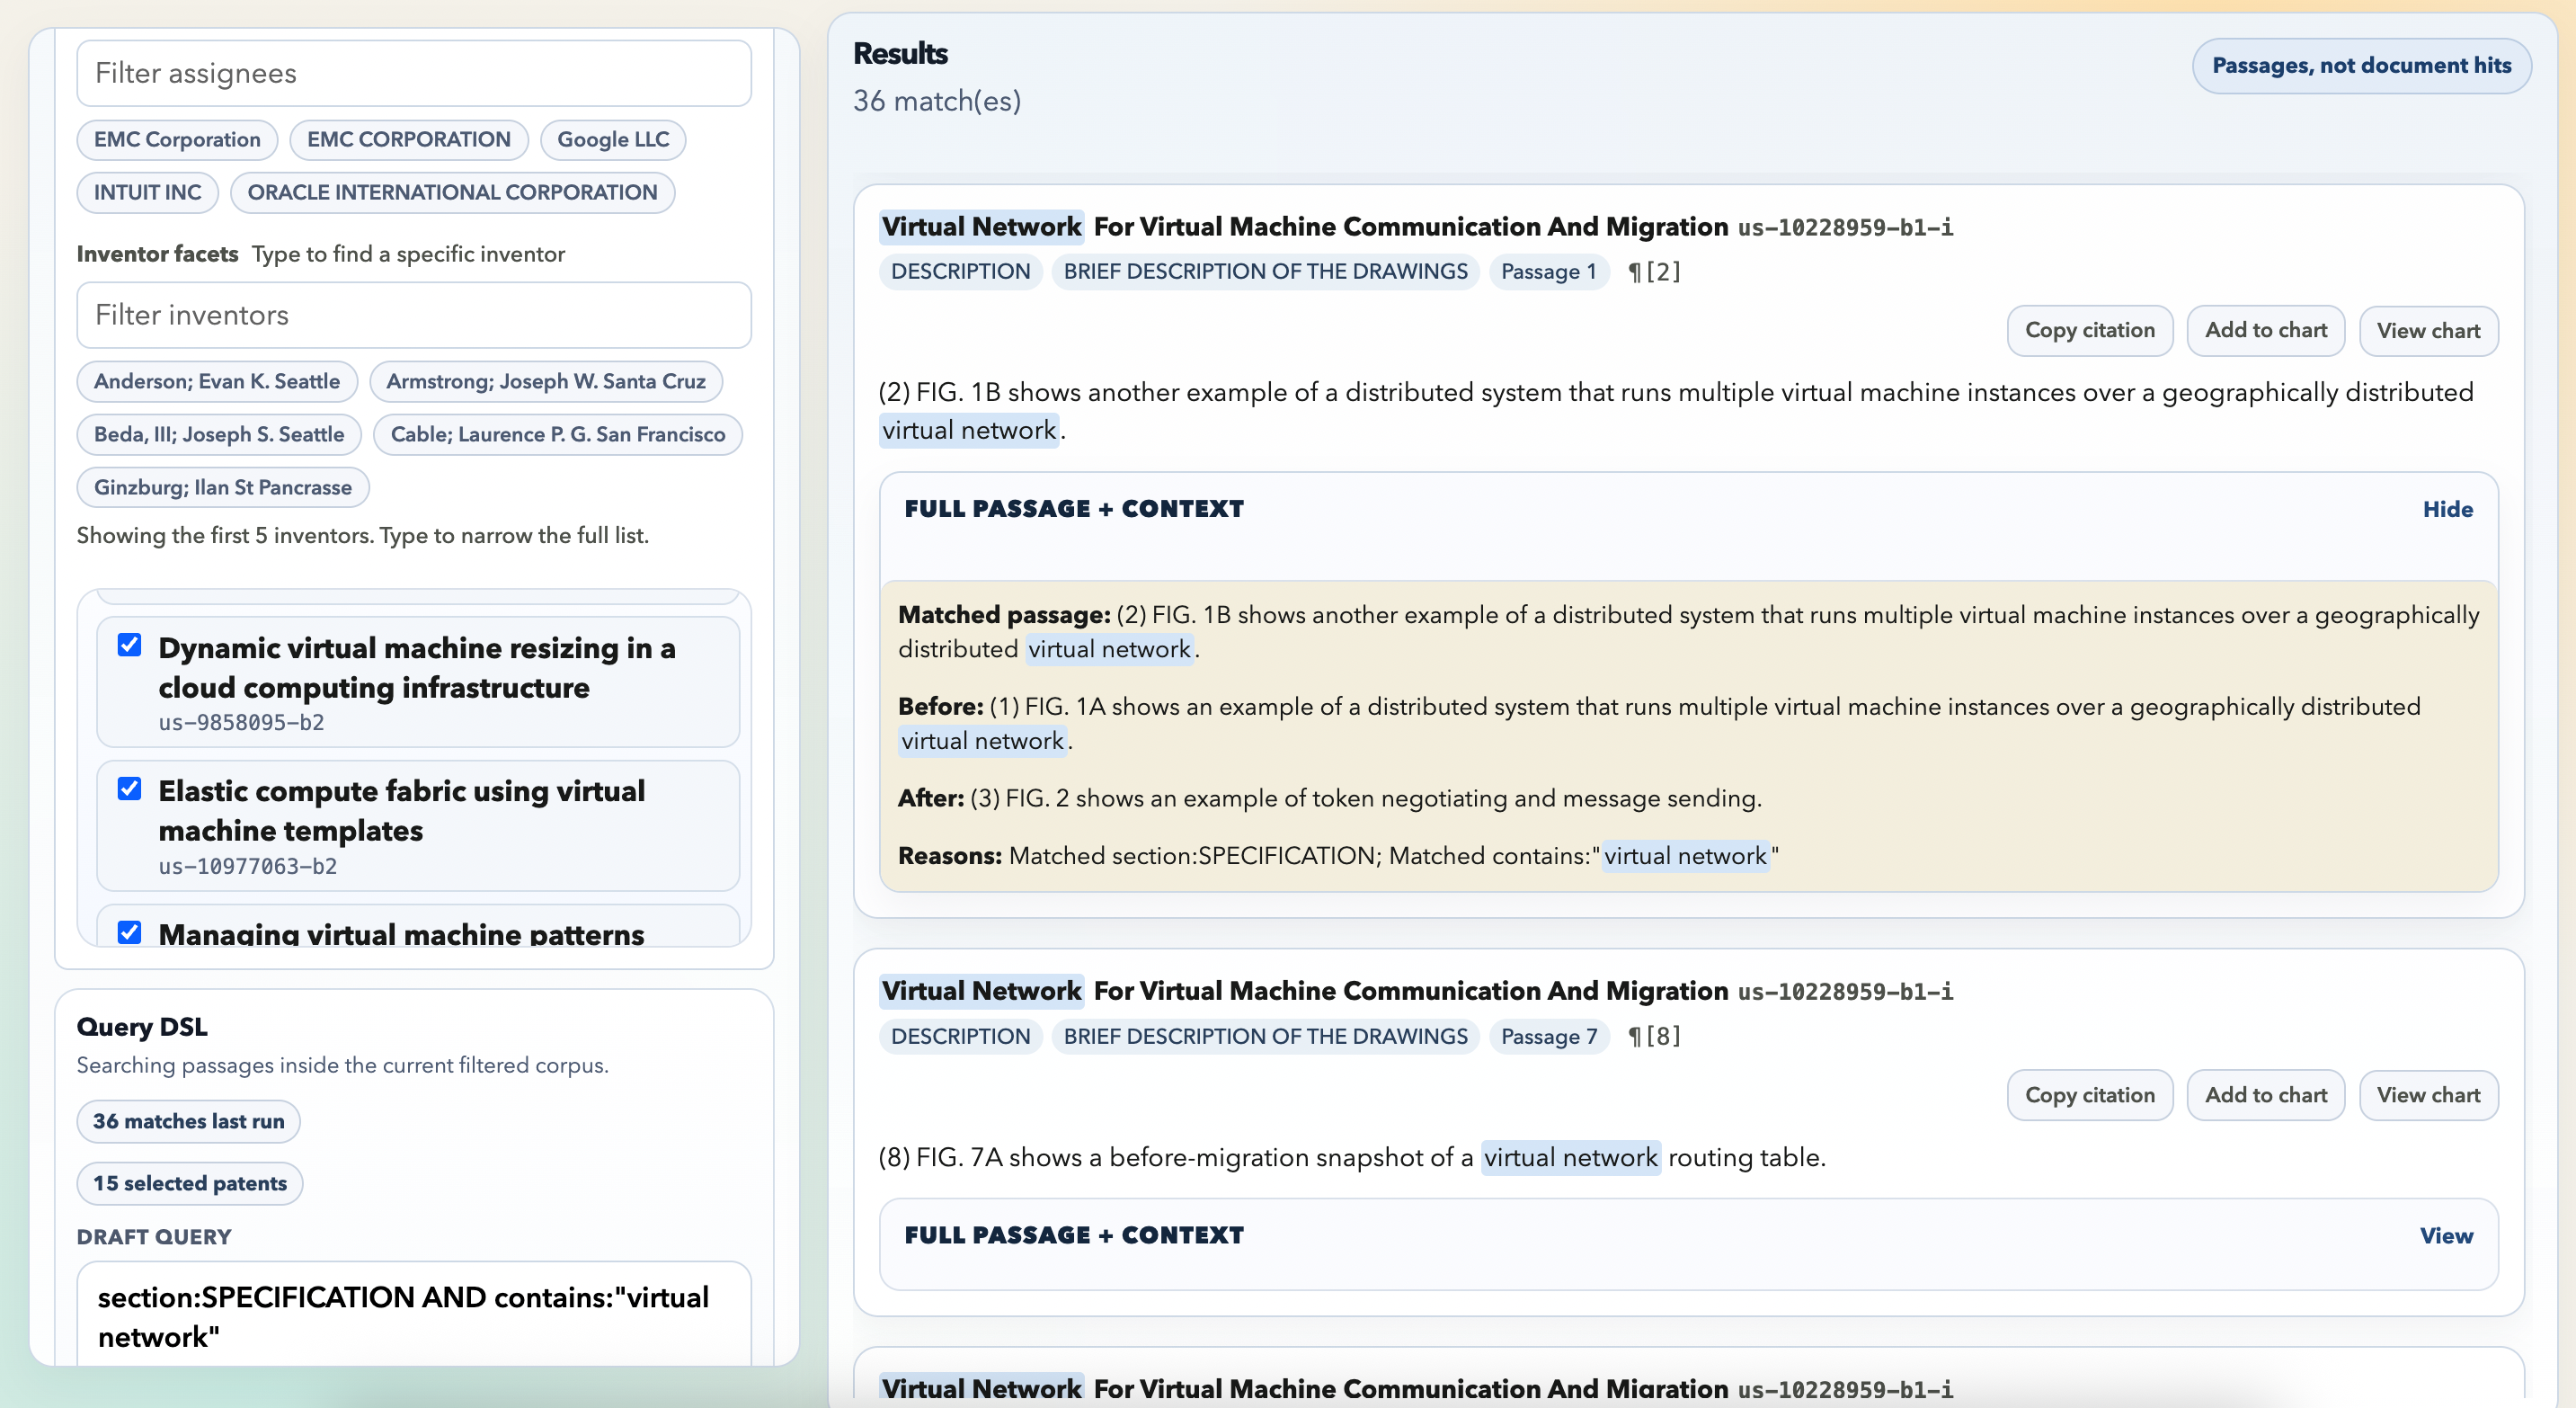
\includegraphics[width=\textwidth]{figures/search-workspace.png}
  \caption{Search workspace for the prototype. The interface keeps corpus scoping, metadata facets, DSL query authoring, and passage-level results visible in one surface so an examiner can iteratively refine the search space, inspect local context around each hit, and preserve citation-ready evidence without reopening full patent documents in a separate viewer.}
  \Description{A wide screenshot of the search workspace. The left side shows a document manager and metadata filters for scoping the active corpus. The center shows a DSL query editor with a structured patent query. The right side shows passage-level result cards with section labels, surrounding context, and actions for copying citations or saving evidence.}
  \label{fig:search-workspace}
\end{figure*}

\smallskip\noindent\textbf{The abstraction exposed to the user.}
The environment's central abstraction is not ``a better search box.'' It is a
program state composed of three linked parts: a scoped corpus, a query program,
and a set of evidence artifacts. The scoped corpus is the selected patent set
plus its metadata constraints. The query program is the DSL expression that
denotes a set of matching passages over the
\DocSectionPassage{} hierarchy. The evidence artifact is
not just copied text; it preserves the selected passage, its citation anchor,
the source document set, and the query text that produced it. This gives users
something closer to a reusable, inspectable representation
of search intent and search outcome that can move forward into claim-chart
drafting and backward into result reproduction.

The search interface supports both explicit submission and live refinement.
On a fresh page load, the system does not immediately run a broad query across
all selected documents; this avoids hydrating unnecessary documents before the
examiner has begun interacting. Once the examiner edits the query, changes the
document selection, or presses the run button, the interface enables a 600ms
debounced live-refresh loop so subsequent refinements update the result set in
near real time. In parallel, the frontend opportunistically preloads the
currently selected documents so the first query on that selected set need not
hydrate each document one by one.

\smallskip\noindent\textbf{Why this tool, for this population.}
Every major feature in the environment can be justified as a response to a
constraint we derived from contextual inquiry. We therefore organize the design
not as a list of interface features, but as a mapping from observed workflow
breakdowns to design requirements and then to implemented tool responses.


\subsection{Walkthrough: Using the Tool for a Real Claim-Mapping Task}

To make the design concrete, we walk through a task modeled on one we observed
in session P03. P03 was evaluating a software patent application whose claim
required a mechanism for \emph{dynamic routing table updates}. The task was not
simply to find documents that mentioned routing tables. P03 needed to identify
which candidate references were legally admissible, determine whether the
relevant teaching appeared in the specification rather than only in the claims
or abstract, inspect the surrounding context of each hit, and then preserve the
best evidence for claim mapping. In the observed workflow, these steps were
spread across repeated document opening, repeated \texttt{Ctrl+F} searches,
manual filing-date checks, and handwritten or Word-based notes.

With our tool, the examiner begins by loading the candidate references into the
search workspace and making the active corpus explicit. They can narrow the
working set before close reading by combining metadata and classification
constraints directly in the same query state that will later drive passage
retrieval:

\Needspace{7\baselineskip}
\begin{lstlisting}[caption={Scoping a legally admissible technical slice before close reading.}]
meta.filingDate:<2018-03-15 AND cpc:"H04L 45/00"
\end{lstlisting}

This first step is the direct design response to Need~2. Instead of opening
every candidate reference to inspect dates manually, the examiner can keep the
admissibility constraint attached to the active corpus and revise it as new
references are added or removed.

Once the corpus is scoped, the examiner searches for the claim element itself.
Rather than running a separate search for each synonymous phrase, the examiner
can express the synonym set and section restriction in one query over the
selected documents:

\Needspace{9\baselineskip}
\begin{lstlisting}[caption={Passage-level query for a claim element across a scoped corpus.}]
section:SPECIFICATION AND
  (contains:"routing table"
   OR contains:"forwarding table"
   OR contains:"FIB"
   OR contains:"routing cache")
\end{lstlisting}

The result is not a ranked list of documents but a list of matching passages.
Each card exposes the section type and heading, the paragraph or claim anchor
if present, and the immediately neighboring passages. This is how the tool
addresses Need~4 in use: the examiner can judge whether a hit occurs in the
right part of the patent and whether the surrounding discussion actually
supports the claimed mechanism, without reconstructing that context manually in
another viewer. If a passage looks promising, the examiner can copy a citation
trace or add the result directly to the claim-chart workspace.

The task then continues into synthesis rather than stopping at retrieval. When
the examiner adds a result to the chart, the system preserves the passage, its
anchor, the source document IDs, and the query text that produced it. The chart
workspace groups evidence under claim elements and keeps the rows editable, so
the examiner can continue building a claim chart without losing the provenance
of how each piece of evidence was found. This is the design response to Need~3:
the handoff from search to claim mapping is treated as part of the same
workflow rather than as a manual export into Word or paper notes.
Figure~\ref{fig:claim-chart-workspace} shows this downstream workspace, where
saved evidence remains grouped, editable, and linked back to the originating
search state.

\begin{figure*}[t]
  \centering
  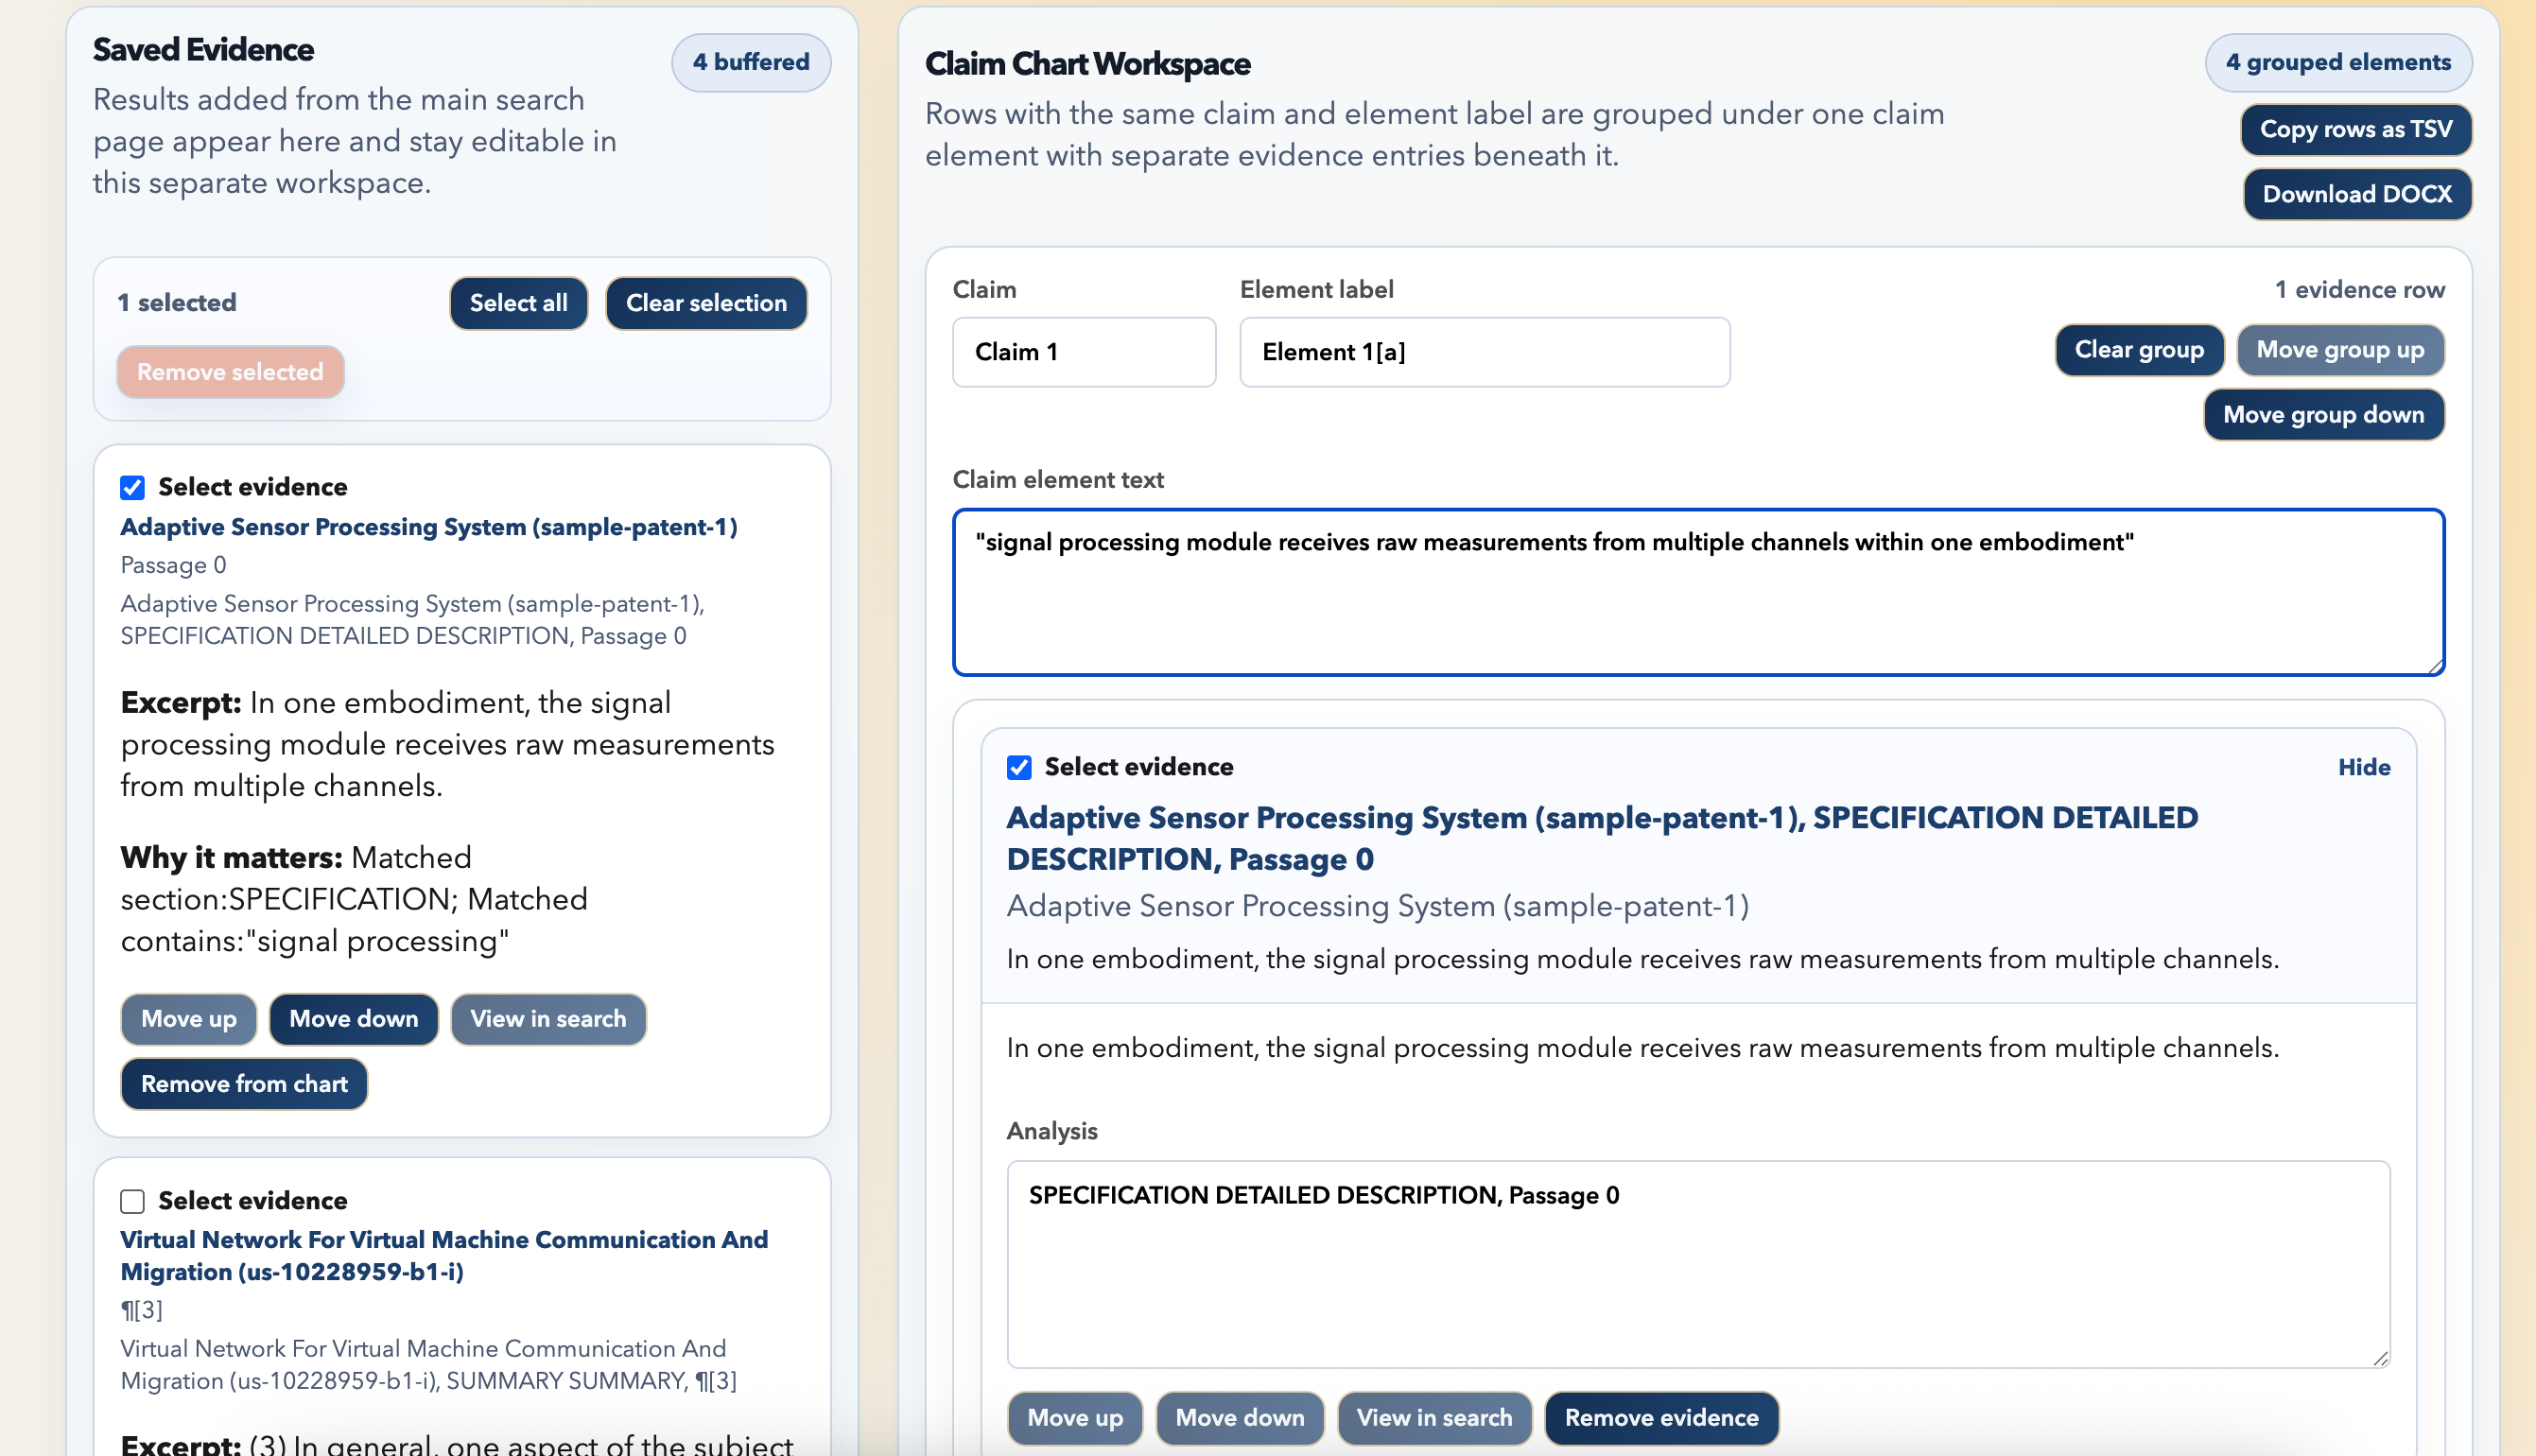
\includegraphics[width=\textwidth]{figures/claim-chart-workspace.png}
  \caption{Claim-chart workspace for the prototype. Evidence selected during search remains available as the examiner drafts grouped claim-chart rows, edits element text, and exports the resulting chart, making the handoff from retrieval to downstream synthesis part of the same interactive workflow.}
  \Description{A wide screenshot of the claim-chart workspace. A saved-evidence panel on the left lists passages carried forward from search. The main panel on the right shows editable claim-chart fields, grouped claim elements, and evidence rows that can be exported as a chart.}
  \label{fig:claim-chart-workspace}
\end{figure*}

Finally, if the result set contains false positives, the examiner can refine
the query incrementally instead of restarting the search process. For example,
if the synonym-expanded result set still mixes dynamic rerouting with static
configuration text, the examiner can add a negative constraint directly to the
same query program:

\Needspace{9\baselineskip}
\begin{lstlisting}[caption={Refining a noisy result set with explicit exclusion.}]
section:SPECIFICATION AND
  (contains:"routing table"
   OR contains:"forwarding table"
   OR contains:"FIB") AND
  NOT contains:"static route"
\end{lstlisting}

The debounced live-refresh loop shows the effect of that change immediately,
so the examiner can appraise whether the new constraint removed false positives
without restarting the workflow. The same language also composes structural
anchors with content constraints when the task shifts from broad retrieval to
pinpoint support for a particular claim element:

\Needspace{8\baselineskip}
\begin{lstlisting}[caption={Combining claim anchors with content constraints.}]
claim:8 AND
  (contains:"routing cache"
   OR contains:"forwarding table")
\end{lstlisting}

This behavior is the concrete realization of Need~5: search remains an
iterative appraise-and-refine process, but one in which the search state,
evidence, and downstream charting artifacts stay linked throughout.

This walkthrough also illustrates how the four design decisions fit together in
practice. The examiner first scopes a working corpus, then queries over patent
structure, then refines the search through a composable DSL, and finally carries
evidence forward with provenance intact. That sequence is what the tool is
designed to support.


\subsection{Decision 1: Make the active corpus explicit before close reading}

\emph{Observation from need-finding.} Participants did not begin by deeply
reading every candidate reference. They first narrowed a working set by
classification, assignee, inventor, date, or prior familiarity, then returned
to that subset while refining the search. P03 described manually checking
filing dates across candidate references, and several participants described
keeping track of ``the references I am actively working with'' in ad hoc ways.

\emph{Design requirement.} Corpus state had to become a first-class part of
the interaction rather than background setup. The user needed an explicit,
revisable working set before paying the cost of passage-level inspection.

\emph{Implemented response.} The search workspace exposes an explicit selected
patent set, metadata facets, and DSL predicates such as \texttt{cpc:} and
\texttt{meta.filingDate:}. The backend indexes lightweight metadata eagerly
while deferring full passage hydration until a document is selected or queried.
This couples the interface decision to a systems decision: corpus scoping stays
cheap, while expensive document loading is delayed until it supports an actual
examiner action.

The same idea appears in the query language. An examiner can constrain the
working set to a legally admissible slice before reading passages:

\Needspace{7\baselineskip}
\begin{lstlisting}[caption={Constrain a scoped corpus by filing date and CPC.}]
meta.filingDate:<2018-03-15 AND cpc:"H04L 45/00"
\end{lstlisting}

This is the design response to Need~2. Instead of opening candidate references
one by one to inspect dates, the examiner can keep admissibility constraints in
the same state as the selected corpus and revise them as the search evolves.


\subsection{Decision 2: Preserve patent structure in the retrieval model}

\emph{Observation from need-finding.} Participants described their information
needs in terms of sections and citeable locations, not whole documents. P05
wanted hits in the background and detailed description rather than the abstract
or claims, while P01 emphasized the effort required to recover the exact
paragraph-level location needed for citation.

\emph{Design requirement.} The retrieval unit had to be smaller than the full
document and had to preserve enough structure for relevance judgment, citation,
and reuse. This meant modeling patents in the same units examiners actually use
when talking about evidence.

\emph{Implemented response.} We represent each patent as a
\DocSectionPassage{} hierarchy. A \texttt{Document}
stores metadata such as filing date, assignee, inventors, and CPC codes. A
\texttt{Section} carries a canonical type drawn from a closed vocabulary such
as \textsc{background}, \textsc{specification}, or \textsc{claims}. A
\texttt{Passage} is the smallest retrieval unit and can carry anchors such as
\texttt{paragraphId}, \texttt{claimNo}, and figure references. The result card
then surfaces section type, heading, anchors, and neighboring passages so the
examiner can judge relevance without reconstructing that structure manually.

This design choice also explains why section type is a dedicated predicate
rather than an arbitrary metadata field. Participants referred to legal section
roles, not heading substrings. P05 asked for hits ``in the background and
description sections, not in the abstract or claims,'' so the model normalizes
those section roles at parse time and exposes them directly in the query
language:

\Needspace{7\baselineskip}
\begin{lstlisting}[caption={Section-scoped containment query.}]
section:SPECIFICATION AND contains:"virtual machine migration"
\end{lstlisting}

Similarly, paragraph anchors are preserved because citation work depends on
them. By extracting \texttt{paragraphId} at parse time and surfacing it on the
result card, the tool keeps citation-relevant structure available during search
instead of requiring the examiner to reopen the source document.


\subsection{Decision 3: Support transparent iterative refinement with a composable DSL}

\emph{Observation from need-finding.} Participants did not formulate one
perfect query and wait for a ranked list. They iteratively probed the corpus,
expanded synonym sets, added or removed constraints, and revised their search
as they learned more about the art. P02 explicitly described search as
``appraising the art as you search for it, and refining your search based on
that.'' Participants were also frustrated by ranked systems whose behavior did
not reveal how to revise a failing search.

\emph{Design requirement.} The query representation had to be editable,
composable, and interpretable enough that a user could understand why a result
appeared and what to change next. This is where the PL contribution becomes
central: the tool needs a small language whose semantics are tied to patent
structure rather than a black-box retrieval score.

\emph{Implemented response.} The environment uses a textual Boolean DSL with
phrase containment, section predicates, paragraph anchors, CPC filters,
metadata filters, and Boolean composition via \texttt{AND}, \texttt{OR}, and
\texttt{NOT}. A query denotes a set of passages within a scoped corpus, not a
ranked list of whole documents. Internally, the query is parsed into an
expression tree evaluated over the patent hierarchy, and each result card
reports the predicates that matched.

This decision is visible in the simplest search patterns. Need~1 established
that examiners manually enumerate synonyms and rerun separate searches for each
variant, so synonym management becomes ordinary Boolean composition:

\Needspace{9\baselineskip}
\begin{lstlisting}[caption={Synonym expansion across a loaded corpus.}]
section:SPECIFICATION AND
  (contains:"routing table"
   OR contains:"forwarding table"
   OR contains:"FIB"
   OR contains:"routing cache")
\end{lstlisting}

Need~4 established that examiners want section-scoped retrieval and pinpoint
anchors, so the same language also supports predicates such as
\texttt{section:SPECIFICATION}, \texttt{paragraph:42}, and date constraints via
\texttt{meta.filingDate}. Because results expose a match-reason string, each
edit to the query remains inspectable. After the first explicit search, the
workspace enables a debounced live-refresh loop so users can make small local
edits and immediately see whether they narrowed the corpus usefully or removed
too much.

For example, the same query can be narrowed without abandoning the current
search state:

\Needspace{8\baselineskip}
\begin{lstlisting}[caption={Composing metadata, section, and exclusion filters.}]
meta.filingDate:<2018-03-15 AND
  section:SPECIFICATION AND
  contains:"routing table" AND
  NOT contains:"static route"
\end{lstlisting}

We also chose a textual DSL over a GUI-only filter panel because examiners
already work in Boolean query strings and need persistent artifacts they can
reuse later. A query string is not just an interaction state; it is a compact
representation of search rationale that can be saved, shared, and cited again
when the analysis moves downstream.


\subsection{Decision 4: Keep retrieval and claim mapping in one provenance-preserving workflow}

\emph{Observation from need-finding.} Retrieval did not end when a participant
found a promising passage. Participants copied text into Word, personal claim
charts, or paper notes, manually preserved citation details, and often had to
remember which query or document state had produced a passage.

\emph{Design requirement.} The tool had to preserve provenance across the
handoff from retrieval to synthesis and had to treat evidence capture as part
of the same workflow rather than an external afterthought.

\emph{Implemented response.} Each result card includes \texttt{Copy citation}
and \texttt{Add to chart} actions. When a passage is transferred, the system
keeps the selected passage, its anchor, the source document set, and the query
that produced it. The claim-chart workspace then groups evidence under claim
elements, keeps rows editable, and supports export as TSV or DOCX.

This decision is what turns the tool from a retrieval prototype into a workflow
prototype. In the P03-style task we observed, the examiner did not simply need
to find passages mentioning a routing-table concept. They needed to judge those
passages in context, preserve paragraph-level evidence, and organize the
results under a claim element without losing where the evidence came from. The
search workspace therefore presents neighboring context and anchors on the
result card, while the chart workspace preserves those results as evidence
artifacts rather than detached text snippets.

Seen this way, the central design abstraction of the tool is a linked program
state: a scoped corpus, a query program, and a set of evidence artifacts. That
is the connection between the design argument and the implementation argument.
The system is not just returning passages; it is preserving the state needed to
move from search to claim-chart drafting without manual transcription.


%% ====================================================================
%%  SECTION 6 — TECHNICAL CHALLENGES AND SOLUTIONS
%% ====================================================================
\section{Technical Challenges and Technical Solutions}

The hardest implementation problems were not frontend polish or debugging
incidents. They arose from turning a messy, document-centric workflow into a
precise programmable system. In each case, the challenge was to define an
abstraction that both matched examiner reasoning and admitted a concrete
execution strategy. The three hardest challenges were therefore not ``how do we
build the UI'' but: how to give heterogeneous patent sources a common semantic
domain, how to give the query language a compositional meaning over that domain,
and how to make query results persist as reusable evidence rather than
ephemeral hits. Put differently, we needed to decide what the objects of the
system were, what programs over those objects meant, and what a reusable result
of program execution should contain. Those questions are what make the section
feel like PL+HCI rather than ordinary application engineering.

\subsection{Challenge 1: Defining a Source-Independent Semantic Domain}

The first challenge was representational. Patent sources arrive as plain-text
files with explicit section markers and paragraph anchors, or as
text-extractable PDFs whose formatting is noisier and whose logical structure is
only partially visible in the text stream. A passage-level query language is
only meaningful if both sources map into the same internal representation; if
section boundaries, paragraph IDs, or claim passages are format-dependent, then
the language has no stable semantics.

Formally, the problem was to define a normalization procedure from raw patent
sources into a single structured representation such that predicates like
\texttt{section:SPECIFICATION} and \texttt{paragraph:42} would denote the same
kind of object regardless of source format. Without that guarantee, the DSL
would be only surface syntax over a collection of parser-specific heuristics.

A naive solution would have been to keep separate parsing paths for each source
type and let downstream code interpret whatever structure each parser happened
to emit. That would have been easier to prototype, but it would have made the
meaning of structural queries dependent on document format. The deeper
difficulty of this challenge was therefore not text extraction alone; it was
committing to a representation invariant strong enough that the rest of the
system could ignore source-specific details.

Our solution was to normalize all sources into a common
\DocSectionPassage{} hierarchy before query execution.
The parser canonicalizes heading variants into a closed section vocabulary,
splits text into passage units, and annotates each passage with structural
anchors such as \texttt{paragraphId}, \texttt{claimNo}, and figure references
when available. This hierarchy is the semantic domain of the DSL: the same
\texttt{section:SPECIFICATION} query must mean the same thing whether the source
was a USPTO-style text file or a PDF extracted through \texttt{pypdf}. By
solving normalization at parse time, we keep the execution model simple and make
structural predicates stable across heterogeneous inputs. This was the key
invented representational move in the system: instead of searching over raw
documents, we first re-encoded patents into the units examiners actually reason
about.

This choice also shaped the rest of the architecture. Because the normalized
hierarchy is stored as structured JSON rather than reconstructed on every query,
the query engine and evidence layer can operate over one semantic domain even
when the original sources differ substantially. The cost is that parsing becomes
a more semantically loaded stage of the pipeline, but the benefit is that later
stages remain simpler and more predictable.

\subsection{Challenge 2: Giving the DSL a Compositional Meaning}

The second challenge was semantic. The DSL has to combine heterogeneous
predicates---section type, containment, metadata comparisons, CPC filters,
paragraph anchors, claim numbers, and negation---without collapsing back into a
bag of ad hoc special cases. In other words, every well-formed query needs a
clear denotation over passage candidates, and the system needs an internal form
that supports both parsing and execution.

The technical problem here was not merely parsing strings. It was defining an
intermediate representation in which every construct had a local meaning and in
which Boolean composition could be applied uniformly across otherwise different
kinds of predicates. We also needed that representation to support explanation,
because a user must be able to tell why a passage matched and how to revise the
query if the result set is wrong.

Here too, the easy alternative would have been to implement each feature as a
special-case search routine: one path for section constraints, one for metadata,
one for containment, and ad hoc branching for combinations. That style is common
in search tools, but it would have made the language harder to extend, harder to
explain, and harder to treat as a reusable artifact. The technical challenge was
to avoid building a bag of options and instead define a compact language with a
uniform execution model.

We addressed this by compiling surface syntax into an explicit query-expression
tree. Filter clauses become leaf predicates, while Boolean composition becomes
\texttt{and}, \texttt{or}, and \texttt{not} nodes in an internal
representation. Query execution then evaluates that tree over a stream of
candidate passages produced by flattening the parsed document hierarchy. This is
the core PL move in the system: the DSL is not a thin wrapper over API flags,
but a real language with a compositional intermediate representation and an
evaluation procedure. The resulting model lets us explain exactly what a query
means, why a result matched, and how a user should revise the query when the
result set is wrong. In effect, we turned patent search constraints into a
small executable program over structured documents rather than a bundle of
special-purpose search options.

We can state that execution model more formally. Let $P(C)$ be the set of
passages obtained by flattening a scoped corpus $C$ after normalization into
the \DocSectionPassage{} hierarchy. The core syntax of the DSL is:

$$
\begin{array}{rcl}
e & ::= & f \mid \textsf{not}\ e \mid e\ \textsf{and}\ e \mid e\ \textsf{or}\ e \\
f & ::= & \textsf{section}(s) \mid \textsf{contains}(t) \mid \textsf{heading}(h) \\
  & \mid & \textsf{meta}(k, \odot, v) \mid \textsf{cpc}(c) \mid \textsf{paragraph}(p) \\
  & \mid & \textsf{claim}(n) \mid \textsf{figure}(g)
\end{array}
$$

where $s$ ranges over canonical section types,
$\odot \in \{\textsf{eq},\textsf{lt},\textsf{lte},\textsf{gt},\textsf{gte},\textsf{contains},\textsf{startswith}\}$
selects a metadata comparison operator, and the remaining terminals range over
strings or identifiers in the obvious way. In the concrete DSL, the last two
cases correspond to the substring and prefix operators written with
\texttt{\~{}} and \texttt{\string^}. The denotation of a query is a set of
passages:

$$
\llbracket f \rrbracket_C = \{ p \in P(C) \mid f\text{ holds on }p \},
$$

with Boolean structure interpreted compositionally:

$$
\llbracket e_1\ \textsf{and}\ e_2 \rrbracket_C = \llbracket e_1 \rrbracket_C \cap \llbracket e_2 \rrbracket_C,
\qquad
\llbracket e_1\ \textsf{or}\ e_2 \rrbracket_C = \llbracket e_1 \rrbracket_C \cup \llbracket e_2 \rrbracket_C,
$$

$$
\llbracket \textsf{not}\ e \rrbracket_C = P(C) \setminus \llbracket e \rrbracket_C.
$$

This is a small formalism, but it captures the key claim of the section: every
query construct has a local meaning over normalized passages, and composition
is set-theoretic rather than ad hoc.

That decision also supports two downstream properties that matter in practice.
First, it enables the match-reason strings shown in the UI, because the engine
can report which leaf predicates succeeded under which Boolean context. Second,
it gives the language a stable place to grow. Future constructs such as richer
synonym operators or admissibility predicates can be added as new expression
forms rather than bolted on as one-off UI features.

\subsection{Challenge 3: Reifying Search Results as Reusable Evidence}

The third challenge was to make query results reusable as evidence rather than
ephemeral hits. A matched passage is only useful if the examiner can inspect
its local context, recover its citeable location, and later reproduce how it was
found. Traditional search interfaces treat result presentation and downstream
note-taking as separate problems; our tool needed a single representation that
could serve both.

The formal problem was to define a result object rich enough to support three
different operations at once: immediate relevance judgment, later citation, and
downstream reuse in claim mapping. A bare text snippet is insufficient for all
three, because it omits the structural anchor, the surrounding context, and the
query state that produced it.

This challenge is easy to underestimate because conventional systems usually
split it across products: search returns a hit, and some other tool handles
notes, citation, or authoring. Our study suggested that this split is itself a
source of breakdown. Once a useful passage leaves the search interface, the user
immediately loses the conditions under which it was found and must reconstruct
that meaning manually. The technical challenge was therefore to define an
evidence object that remains meaningful outside the moment of retrieval.

Our solution was to preserve provenance end to end. Each query match carries its
document ID, section type, section title, passage index, optional paragraph or
claim anchor, neighboring context, and a set of human-readable reason strings
derived from the predicates that matched. When a user adds a result to the
claim-chart workspace, the stored chart row also records the source query text,
source document IDs, and result key. This turns evidence capture into a
programmable artifact rather than a transcription step: a row in the chart is
not only an excerpt but also a reference back to the executable query state that
produced it. That provenance-preserving representation is what makes the search
and synthesis workflow inspectable and reversible. The key solution was to
treat provenance as part of the data model, not as logging metadata layered on
after retrieval.

Again, the point can be stated formally. A query match is not modeled as a bare
string, but as a structured value

$$
\mathit{Match} = \left\langle
\begin{array}{l}
\mathit{passageId},\ \mathit{documentId}, \\
\mathit{sectionType},\ \mathit{sectionTitle}, \\
\mathit{passageIndex},\ \mathit{passageText}, \\
\mathit{contextBefore},\ \mathit{contextAfter}, \\
\mathit{reasons},\ \mathit{paragraphId?}, \\
\mathit{claimNo?},\ \mathit{figureRefs?}
\end{array}
\right\rangle
$$

and the evidence object carried into downstream synthesis extends that value
with the program state that produced it:

$$
\begin{array}{rcl}
\mathit{Evidence} & = & \mathit{Match} \times \mathit{QueryText} \\
& & \times\ \mathcal{P}(\mathit{DocumentId}) \\
& & \times\ \mathit{ResultKey}
\end{array}
$$

This typing decision is what makes the reuse story precise. Evidence is not
``text plus notes''; it is a result value paired with enough provenance to be
rechecked, regrouped, or exported without severing it from the query execution
that produced it.

This is also where the system stops being only a retrieval tool. Once result
objects preserve enough state to be cited, revisited, and reorganized under
claim elements, they become domain artifacts in their own right. That move is
what connects the PL framing of explicit program state to the HCI observation
that examiners are currently forced to externalize too much of their reasoning
by hand.

\subsection{Remaining Work}

The prototype is still incomplete in three technically important ways. First,
legal admissibility is approximated through derived date fields rather than a
full model of continuation, provisional, and priority relationships, so the
metadata layer still falls short of the legal reasoning examiners sometimes
perform manually. Second, synonym support currently depends on explicit Boolean
enumeration, curated term sets, and optional synonym hooks; a richer construct
for soft matching remains to be designed if we want to preserve transparency
without forcing every expansion into hand-written \texttt{OR} clauses. Third,
the claim-chart workspace preserves provenance, but claim-element grouping and
evidence reuse are still encoded mainly in UI state rather than in a more
explicit programmable representation. Those remaining gaps point to the next
step for the project: extending the language and data model so that more of the
examiner's downstream reasoning becomes first-class rather than remaining
implicit in the interface.

A fourth open issue is scale. The current prototype is designed for an MVP-sized
corpus and relies on lightweight metadata indexing, deferred document
hydration, and passage-level evaluation over selected documents. Extending this
model to much larger corpora while preserving interactive query latency would
require more aggressive indexing and caching strategies, but those strategies
would also need to preserve the same passage-level semantics and provenance
model that make the current system explainable. In that sense, scaling the tool
is not only a systems problem; it is also a representation problem.


%% ====================================================================
%%  SECTION 7 — IMPLEMENTATION
%% ====================================================================
\section{Implementation}

The prototype is implemented as a Python~3 backend and a React/TypeScript
frontend. The backend uses FastAPI and loads parsed patents into an in-memory
document store on startup, then exposes endpoints for health checks, document
listing, document preloading, raw-file parsing, synonym-set inspection, and DSL
query execution. Raw sources in \texttt{backend/data/raw/} are converted into
structured JSON documents in \texttt{backend/data/parsed/} through a parser
pipeline built on \texttt{pypdf} for text-extractable PDFs and custom patent
text parsing logic for section, paragraph, and claim extraction. Query strings
are parsed by a custom recursive-descent parser into an internal expression
tree and then evaluated by the query engine over flattened passage candidates
drawn from the normalized \DocSectionPassage{}
representation. The frontend is built with React~18, TypeScript, and Vite and
acts as a thin client over the backend APIs, providing document selection,
query editing, live refinement, result inspection, and claim-chart management;
the chart export path uses the \texttt{docx} package to generate lightweight
office-action-style artifacts.

We also implemented pytest-based unit tests for the DSL parser, patent parser,
query engine, source loader, synonym-set logic, store behavior, and API
surface. The current prototype supports plain-text and text-extractable PDF
patents; image-only scanned PDFs still require OCR as a preprocessing step. The
full implementation, setup instructions, and supporting documentation are
publicly available at \url{https://github.com/shanayamalik/cs294-sp26}.


%% ====================================================================
%%  SECTION 8 — DISCUSSION
%% ====================================================================
\section{Discussion}

The main lesson from this project is that the PL contribution is not merely
``adding a DSL'' to an existing interface. The deeper intervention is to choose
an abstraction boundary that matches the domain task. By re-representing patent
documents as structured objects and by making sections, passages, anchors, and
metadata queryable values, we created operations that flat document-level
search cannot express cleanly. For future implementers, the practical lesson is
to begin by asking what objects users actually reason about in their work, not
what objects an existing tool or storage format happens to expose. In our case,
the decisive move was to model patents as
\DocSectionPassage{} rather than as opaque text. A concrete mistake a future
tool builder could make is to accept the storage format as the semantic model:
index whole documents, attach section labels as lightweight metadata, and then
try to recover passage-level behavior later with special cases in the ranking
or UI layer. Our experience suggests that this fails quickly. Once the system's
real unit is still ``document,'' queries like ``find specification passages
with a citeable anchor and local context'' become awkward exceptions instead of
ordinary programs. A more reliable design move is to test the representation
before polishing the interface: write down three domain queries users actually
need, and check whether the core data model can express them directly without
 fallback logic. If it cannot, the abstraction boundary is probably wrong.

The second lesson is that retrieval and synthesis should often be treated as a
single programmable workflow rather than two disconnected products. Existing
systems return ranked documents and then rely on users to externalize
everything that matters afterward: the exact passage, the citation anchor, the
query that found it, and the claim element it may support. Our evidence-capture
workflow suggests that these are not merely downstream usability conveniences;
they are part of the same representation problem. For tool builders, this means
that a result object should be designed for reuse, not just display. Once a
result is modeled as \emph{passage + provenance + query context}, it can move
into a claim chart without losing the semantics of how it was obtained. Here the
concrete failure mode is to treat a result as a display-only snippet: some text
to render on screen, perhaps with a document title and a hyperlink, but nothing
that survives once the user copies it elsewhere. We saw why that breaks the
workflow. The moment the snippet leaves the search page, the user must manually
reconstruct why it matched, where it came from, and whether it still belongs to
the active corpus. Future builders should therefore define the result object as
if it will be consumed by a second tool, even when that second tool is part of
the same product. In practice, that means preserving at least the passage,
anchor, source document identity, query text, and a stable result key. If a
downstream workflow cannot answer ``why do I still trust this snippet?'' then
the result representation is too thin.

The third lesson is methodological. Contextual inquiry did not just suggest UI
features; it shaped the language design itself. Section-scoped predicates,
Boolean composition, passage granularity, and provenance-carrying evidence rows
all came from observed workflow constraints. Without that grounding, it would
have been easy to build a more conventional full-text search interface or an
opaque semantic-search layer. The broader lesson for future implementers is
that need-finding should not stop at feature prioritization. It can and should
inform what the language denotes, what counts as a stable intermediate
representation, and what kinds of execution behavior users will find
interpretable. A practical way to use this lesson is to trace one real task all
the way through and mark every point where the user has to carry state manually
from one representation to another. Those handoffs are often a better guide to
language or environment design than a wish list of features. In our case, the
important observations were not just ``users want better search'' but ``users
manually carry forward synonym sets, admissibility decisions, passage context,
and claim-mapping evidence.'' That is what justified the query language, the
structured document model, and the provenance-carrying result object. Future
builders should be skeptical of any language feature that cannot be traced back
to an observed coordination problem in real work.

A fourth lesson concerns transparency. In domains where expert users revise
their search strategy as they learn, a tool should help them inspect and modify
the search state rather than hide it behind a scoring model they cannot reason
about. Our use of an explicit Boolean DSL and match-reason reporting was not a
rejection of all richer retrieval methods; it was a design choice motivated by
the need for local, comprehensible edits. Future implementers of interactive
languages or environments should therefore treat explainability as a property of
the underlying representation and execution model, not just as a layer of UI
explanation pasted on after the fact. The concrete mistake here is to build an
opaque ranking or semantic-search component and then try to patch over it with
highlighted keywords, confidence badges, or post hoc explanation text. That may
decorate the output, but it does not tell the user what to change next. Our
experience during implementation added one further point that the study alone
did not reveal. We expected match-reason strings to be a lightweight
explanatory convenience, but in practice they changed how query revision felt.
When a result carried explicit reasons such as a section match, a metadata hit,
or a particular containment predicate, it became much easier to tell whether a
bad result set came from an overbroad synonym expansion, an overly narrow
structural constraint, or a corpus-selection mistake. That is a different kind
of benefit than the one surfaced directly by contextual inquiry: it is not just
that users want transparency in the abstract, but that predicate-level reasons
can turn failed searches into diagnosable states during actual use. Future tool
builders should therefore think of explanation not only as a user-facing trust
feature, but as a debugging aid for interactive search itself. The most useful
explanations were the ones that exposed exactly which parts of the executable
query state had succeeded, because those were the explanations that made the
next revision obvious.

More broadly, we expect the same approach to matter beyond patents. Many expert
document domains---regulatory filings, scientific literature, case law, safety
reports---combine rich internal structure with downstream evidence work. In such
domains, a useful programming intervention may not look like general-purpose
automation. It may instead look like a domain-specific representation, a small
query language over that representation, and artifacts that preserve query
provenance as work moves downstream. The central takeaway from this project is
therefore not patent-specific: when expert work depends on structured documents,
iterative interpretation, and evidentiary reuse, the most valuable tool may be
one that makes the underlying work state explicit, programmable, and portable.


%% ====================================================================
%%  SECTION 9 — WHAT ELSE SHOULD YOU KNOW?
%% ====================================================================
\section{Additional Notes}

\subsection{What Changed in a P03-Style Task}

The clearest way to understand what we learned from building the prototype is
not to restate the mapping from needs to features, but to compare how one of
our observed tasks changes when it is replayed inside the system. Consider the
P03-style task used in Section~5: identify prior art relevant to a claim about
dynamic routing table updates, verify that candidate references are legally
usable, inspect whether the teaching appears in the right part of the patent,
and preserve the best evidence for claim mapping. In the observed workflow,
those operations were spread across several loosely connected representations:
search results, open patent documents, manual filing-date checks, ad hoc notes,
and a separate claim-mapping artifact. Replaying the same task with the
prototype made it clear that the primary benefit of the design is not faster
typing or prettier retrieval results. It is the removal of several brittle
state transitions that previously forced the examiner to reconstruct context by
hand.

In the old workflow, the first phase was corpus construction. P03 would gather
candidate references from document-level search, then inspect them one by one
to determine whether any were even admissible under the application's filing
date. That meant the active corpus existed mostly in the examiner's head or in
transient search history. In our prototype, this phase becomes explicit program
state. The candidate set, metadata constraints, and query text all live in one
place, so corpus construction is no longer a hidden precondition for the real
work; it is part of the same inspectable artifact. Using the system ourselves
made that shift feel more important than we expected. Much of the friction in
the original workflow came from losing track of which references were still in
play after several rounds of triage, not merely from the cost of typing date
filters.

The second phase was interpretive inspection. In the old workflow, once P03 had
a promising document, they still had to open it, run local searches, jump among
sections, and decide whether the relevant teaching occurred in the
specification, claims, or some less useful region. That meant relevance was not
judged at the moment of retrieval; it was judged only after a second round of
navigational labor. Replaying the task in the prototype showed why the
passage-level representation matters so much. Because result cards already carry
section type, local context, and anchors, the examiner can make the first
relevance judgment earlier and with less reconstruction. In practice, this did
not eliminate close reading; rather, it moved the first meaningful judgment
closer to the retrieval step, which is exactly where the earlier tools were
weakest.

The third phase was externalization. In the observed workflow, once P03 found a
useful passage, the passage effectively left the search system. It was copied
into notes or a claim chart, and its connection to the query, corpus state, and
surrounding context became fragile. That break was easy to underestimate until
we used the prototype end to end. What mattered was not just that the chart
workspace stored text; it was that the evidence object kept enough provenance to
remain meaningful after the moment of retrieval. This made the downstream chart
feel less like a fresh authoring task and more like a continuation of the same
analysis state. In other words, the prototype taught us that the real boundary
in patent examination is not between search and writing, but between states
that preserve evidence provenance and states that discard it. One further
surprise was that the claim-chart workspace did more than hold evidence after
the fact. We initially treated it as a destination for saved passages, but in
actual use it also became a diagnostic surface: once passages were grouped under
claim elements with their provenance intact, it became much easier to see when
two snippets were really duplicating the same support, when an element still had
no convincing evidence, or when a passage that looked persuasive in isolation
was too weak once placed next to competing support. That was not something the
study alone made fully visible. Building the end-to-end workflow showed that the
synthesis surface can reveal gaps and redundancy earlier, rather than merely
recording conclusions reached elsewhere.

This comparison also clarified what the prototype still does not solve. The
system makes corpus state, query state, and evidence state much more explicit,
but legal admissibility is still only approximated through available metadata;
synonym support still requires hand-authored expansions or curated term sets;
and the claim-chart workspace is still lighter-weight than the full reasoning
structure examiners eventually produce. Those remaining gaps are easier to name
precisely after replaying the P03-style task in the tool, because we can now
say which transitions have been collapsed successfully and which ones still leak
manual work. That, more than any one feature, is what we learned from building
and using the prototype ourselves: the most valuable interventions were the ones
that turned previously implicit workflow state into something explicit,
inspectable, and reusable.

\subsection{Limitations and Threats to Validity}

Several limitations constrain how strongly this prototype should be interpreted.
First, the system has been informed by contextual inquiry and implemented as a
working prototype, but it has not yet been evaluated through a follow-up study
with patent examiners using the full tool in practice. As a result, the paper
can support claims about observed workflow needs, about the design rationale of
the prototype, and about the technical properties of the implementation, but it
cannot yet support strong claims about productivity gains, preference, or
long-term adoption. Second, the participant pool is small and focused on
technical patent examination. That is appropriate for a need-finding study, but
it means the findings should be interpreted as design-relevant observations for
this domain rather than as a comprehensive account of all patent examination
practice.

Third, the current parser pipeline has the limitations of its source material.
Plain-text patents with visible section markers and paragraph anchors are the
best-supported case. Text-extractable PDFs are also supported, but extraction
quality varies with layout, and image-only scanned PDFs still require OCR
preprocessing outside the current system. Because the system's semantics depend
on accurate section and passage boundaries, parsing fidelity is not just an
implementation nuisance; it directly affects the reliability of structural
predicates and citation anchors. Fourth, the prototype currently operates on a
small parsed corpus. The current design decisions around metadata indexing,
document preloading, and passage-level query execution have worked well enough
for an MVP, but they have not yet been stress-tested at a scale comparable to
production patent search systems.

There is also a methodological limitation worth noting. Our need-finding data
come from observed workflows around public patents and reconstructed search
activity, not from direct instrumentation of proprietary examiner systems under
live production conditions. That was the right choice for access and ethics, but
it means there are likely additional organizational constraints, collaboration
practices, and policy-driven behaviors that the prototype does not yet model.
For the research community, the main implication is that this work should be
read as a grounded design intervention, not as the final word on patent search
tooling.

\subsection{Broader Relevance Beyond Patents}

Although the prototype is specific to patent examination, the underlying design
pattern is likely to apply more broadly. Many expert document domains combine
three properties that also appear here: documents have meaningful internal
structure, users reason iteratively rather than in one-shot queries, and useful
results must later be reused as evidence or justification in downstream work.
Scientific literature review, regulatory compliance analysis, case-law research,
safety report inspection, and policy analysis all share some version of this
structure. In each of these settings, traditional document retrieval tends to
collapse the domain into ranked blobs, while users actually reason about
sections, excerpts, citations, and chains of interpretation.

The contribution of this project to that broader space is therefore not just a
patent-specific tool. It is the suggestion that a productive intervention may be
to expose the domain's internal document structure as the semantic domain of a
small language, then preserve the resulting query state and evidence objects as
users move downstream. For future researchers, that suggests a concrete recipe:
study how experts segment documents conceptually, encode those units into an
explicit representation, design a language whose predicates target those units,
and ensure that results carry enough provenance to survive beyond the moment of
retrieval. The particular predicates will vary from domain to domain, but the
general architecture may transfer surprisingly well.

\subsection{Future Directions}

The most immediate next step is deeper language support for parts of the patent
workflow that are still only partially modeled. Legal admissibility reasoning is
the clearest example. The current system can express filing-date constraints and
derived metadata fields, but full priority reasoning for continuations,
provisionals, and foreign applications remains outside the language. A second
direction is to design a more principled notion of soft matching. Right now,
synonym expansion is supported through explicit Boolean enumeration and curated
term sets. That is useful and transparent, but it still places much of the
burden on the examiner. A more advanced construct might support controlled
semantic expansion while remaining inspectable enough to preserve the iterative
revision model that participants valued.

A third direction is to make more of the synthesis stage programmable. The
claim-chart workspace currently preserves source query text and document IDs,
but claim-element grouping and evidence reuse are still mostly UI-level
operations. A richer representation for claim elements, limitation structure,
and evidence relationships could extend the system from a provenance-preserving
search environment into a more fully programmable claim-analysis environment.
Finally, scaling remains an open challenge. Passage-level semantics and
provenance-preserving results become more valuable, not less, as corpora grow,
but scaling them requires indexing and caching strategies that do not erase the
very structure that makes the tool interpretable. Future work therefore needs
to treat scalability, semantics, and interaction design as linked problems
rather than separate phases of engineering.

Taken together, these limitations and directions point to a broader research
agenda. The goal is not to replace expert legal-technical judgment with a more
powerful search box. It is to build languages and environments in which the
state of expert document work becomes explicit, inspectable, and reusable. That
is the strongest claim this project makes, and it is the point from which we
hope others can build.


\begin{acks}
We thank Professor Sarah E.\ Chasins for her guidance throughout this
project and the CS~294 course at UC Berkeley. We also thank the ten patent
examiners who generously shared their time, expertise, and workflows with us.
\end{acks}

\begin{thebibliography}{21}

\bibitem{Ko2006}
A.~J. Ko, B.~A. Myers, M.~J. Coblenz, and H.~H. Aung.
\newblock An Exploratory Study of How Developers Seek, Relate, and Collect
  Relevant Information during Software Maintenance Tasks.
\newblock {\em IEEE Trans. Softw. Eng.}, 32(12):971--987, 2006.

\bibitem{Pirolli2005}
P.~Pirolli and S.~Card.
\newblock The Sensemaking Process and Leverage Points for Analyst Technology
  as Identified Through Cognitive Task Analysis.
\newblock In {\em Proc. Int. Conf. Intelligence Analysis}, volume~5.
  MITRE, McLean, VA, 2005.

\bibitem{Marchionini2006}
G.~Marchionini.
\newblock Exploratory Search: From Finding to Understanding.
\newblock {\em Communications of the ACM}, 49(4):41--46, 2006.

\bibitem{White2009}
R.~W. White and R.~A. Roth.
\newblock {\em Exploratory Search: Beyond the Query-Response Paradigm}.
\newblock Morgan \& Claypool, 2009.

\bibitem{Hearst2009}
M.~A. Hearst.
\newblock {\em Search User Interfaces}.
\newblock Cambridge University Press, 2009.

\bibitem{Bates1989}
M.~J. Bates.
\newblock The Design of Browsing and Berrypicking Techniques for the Online
  Search Interface.
\newblock {\em Online Review}, 13(5):407--424, 1989.

\bibitem{Kuhlthau1991}
C.~C. Kuhlthau.
\newblock Inside the Search Process: Information Seeking from the User's
  Perspective.
\newblock {\em Journal of the American Society for Information Science},
  42(5):361--371, 1991.

\bibitem{Ellis1989}
D.~Ellis.
\newblock A Behavioural Approach to Information Retrieval System Design.
\newblock {\em Journal of Documentation}, 45(3):171--212, 1989.

\bibitem{Russell1993}
D.~M. Russell, M.~J. Stefik, P.~Pirolli, and S.~K. Card.
\newblock The Cost Structure of Sensemaking.
\newblock In {\em Proc. CHI '93}, pages 269--276. ACM, 1993.

\bibitem{Lupu2013}
M.~Lupu, K.~Mayer, N.~Kando, and A.~J. Trippe.
\newblock {\em Current Challenges in Patent Information Retrieval},
  volume~29 of {\em The Information Retrieval Series}.
\newblock Springer, 2013.

\bibitem{Piroi2011}
F.~Piroi and V.~Zenz.
\newblock Evaluating Information Retrieval in the Intellectual Property
  Domain: The CLEF-IP Campaign.
\newblock In {\em Multilingual Information Access Evaluation I. Text Retrieval
  Experiments}, pages 87--108. Springer, 2011.

\bibitem{Magdy2010}
W.~Magdy, J.~Leveling, and G.~J.~F. Jones.
\newblock Exploring Structured Documents and Query Formulation Techniques for
  Patent Retrieval.
\newblock In {\em Multilingual Information Access Evaluation I. Text Retrieval
  Experiments}, pages 410--417. Springer, 2010.

\bibitem{Mahdabi2013}
P.~Mahdabi and F.~Crestani.
\newblock The Effect of Citation Analysis on Query Expansion for Patent
  Retrieval.
\newblock {\em Information Retrieval}, 17(5--6):412--429, 2013.

\bibitem{Storey1999}
M.-A.~D. Storey, F.~D. Fracchia, and H.~A. M{\"u}ller.
\newblock Cognitive Design Elements to Support the Construction of a Mental
  Model during Software Exploration.
\newblock {\em J. Systems and Software}, 44(3):171--185, 1999.

\bibitem{Nersessian2008}
N.~J. Nersessian.
\newblock {\em Creating Scientific Concepts}.
\newblock MIT Press, 2008.

\bibitem{Beyer1997}
H.~Beyer and K.~Holtzblatt.
\newblock {\em Contextual Design: Defining Customer-Centered Systems}.
\newblock Morgan Kaufmann, 1997.

\bibitem{Lubin2021}
J.~Lubin and S.~E. Chasins.
\newblock How Statically-Typed Functional Programmers Write Code.
\newblock {\em Proc. ACM Program. Lang.}, 5(OOPSLA):Article 155, 2021.

\bibitem{Zhang2020}
T.~Zhang, B.~Hartmann, M.~Kim, and E.~Paez.
\newblock Enabling Data-Driven API Design with Community Usage Data:
  A Need-Finding Study.
\newblock In {\em Proc. CHI '20}, pages 1--13. ACM, 2020.

\bibitem{Braun2006}
V.~Braun and V.~Clarke.
\newblock Using Thematic Analysis in Psychology.
\newblock {\em Qualitative Research in Psychology}, 3(2):77--101, 2006.

\bibitem{Chamberlin1974}
D.~D. Chamberlin and R.~F. Boyce.
\newblock SEQUEL: A Structured English Query Language.
\newblock In {\em Proc. ACM SIGFIDET Workshop on Data Description, Access and
  Control}, pages 249--264. ACM, 1974.

\bibitem{Piwowarski2006}
B.~Piwowarski and G.~Dupret.
\newblock Evaluation in (XML) Information Retrieval: Expected
  Precision-Recall with User Modelling.
\newblock In {\em Proc. SIGIR '06}, pages 260--267. ACM, 2006.

\end{thebibliography}

\end{document}
